

\documentclass[11pt,a4paper]{article}

% Begin preamble
\usepackage[margin=20mm]{geometry}
\usepackage{fontspec}
\IfFontExistsTF{Times New Roman}{\setmainfont{Times New Roman}}{\setmainfont{TeX Gyre Termes}}
\IfFontExistsTF{Arial}{\setsansfont{Arial}}{\setsansfont{TeX Gyre Heros}}
\IfFontExistsTF{Consolas}{\setmonofont{Consolas}}{\setmonofont{Latin Modern Mono}}
\usepackage{graphicx,amsmath,booktabs,tabularx,array,placeins}
\usepackage[font=small,labelfont=bf]{caption}
\usepackage[numbers,sort&compress]{natbib}
\usepackage[hidelinks]{hyperref}
\usepackage{microtype}
\setlength{\parindent}{0pt}
\setlength{\parskip}{.5em}
\linespread{1.08}
\setcounter{tocdepth}{2}
\emergencystretch=2em
\newcommand{\bpm}{\text{breaths/min}}

\usepackage{needspace}

\raggedbottom
\renewcommand{\topfraction}{.98}
\renewcommand{\bottomfraction}{.95}
\renewcommand{\textfraction}{.02}
\renewcommand{\floatpagefraction}{.7}
\setcounter{topnumber}{4}
\setcounter{totalnumber}{6}
\setlength{\textfloatsep}{8pt plus 2pt minus 2pt}
\setlength{\floatsep}{8pt plus 2pt minus 2pt}
\setlength{\intextsep}{8pt plus 2pt minus 2pt}
\makeatletter\setlength{\@fptop}{0pt}\setlength{\@fpsep}{12pt}\setlength{\@fpbot}{0pt plus 1fil}\makeatother

% End preamble
\begin{document}
% Begin cover
\begin{titlepage}
\thispagestyle{empty}
\setlength{\parskip}{0pt}
\linespread{1}\selectfont
\providecommand{\HRule}{\rule{\linewidth}{0.5mm}}
\begin{center}

\includegraphics[width=0.35\textwidth]{figures/uom_banner.png}~\\[0.3cm]
\textsc{\Large Final Report}\\[0.3cm]
\HRule \\[0.3cm]
{\huge\bfseries The Art of Scientific Computing:\\
Project Title: ECG Respiratory Rate\\
From Supplied QRS to GQRS}\\[0.3cm]
\HRule \\[0.8cm]
\begin{minipage}{0.45\textwidth}
\begin{flushleft}\large
\textit{Author:}\\
Kaibo Qiao\\
Student ID: 1652063
\end{flushleft}
\end{minipage}
\begin{minipage}{0.45\textwidth}
\begin{flushright}\large
\textit{Subject Handbook code:}\\
COMP-90072
\end{flushright}
\end{minipage}
\\[1.0cm]

\vspace{1.0cm}
Faculty of Science\\
The University of Melbourne\\[0.5cm]
{\small 27 October 2026}\\[1.5cm]
Subject co-ordinators: A/Prof. Suzie Sheehy \& Prof. Christian Reichardt\\[0.8cm]
\end{center}
\end{titlepage}

% End cover
\pagenumbering{roman}
\section*{Abstract}\addcontentsline{toc}{section}{Abstract}
Breathing changes R-R interval, ECG waveform amplitude, and local voltage, making it possible to derive hints about respiratory rate estimation. The current study employs an ECG signal alongside chest effort measurement data from Apnea-ECG. It starts by deriving respiratory clues via the supplied QRS markers, calculating the rates of cycles and fusing them into an ECG-derived respiratory rate that is compared against a chest-derived reference respiratory rate. Errors are analyzed at the level of the underlying ECG and heartbeat markers. The GQRS method is then employed to derive heartbeats anew while keeping the respiration processing unchanged. Using the Count-adv method, the GQRS based chain yields a smaller MAE overall.
\clearpage{\small\tableofcontents}\clearpage\pagenumbering{arabic}
% Begin body
\section{Introduction}
\subsection{From breathing to respiratory monitoring}
Breathing is a periodic physiological function. During inspiration, air goes into the lungs, while expiration takes the air out of the lungs. Both of these functions make one respiratory cycle, which can be measured in the number of respiratory cycles in one minute. For that purpose, it is useful to begin from the description of how the breath manifests itself physiologically and visually on the record.

Air movements are accompanied by the movements of the chest. When inspiration occurs, the chest expands and the diaphragm below the lungs contracts and descends (Figure~\ref{fig:intro_breathing}). In the course of expiration, these muscles relax, and the volume of the chest becomes smaller. The pressure differences produced by such movements allow air to go in and out of the lungs.
\begin{figure}[!htbp]\centering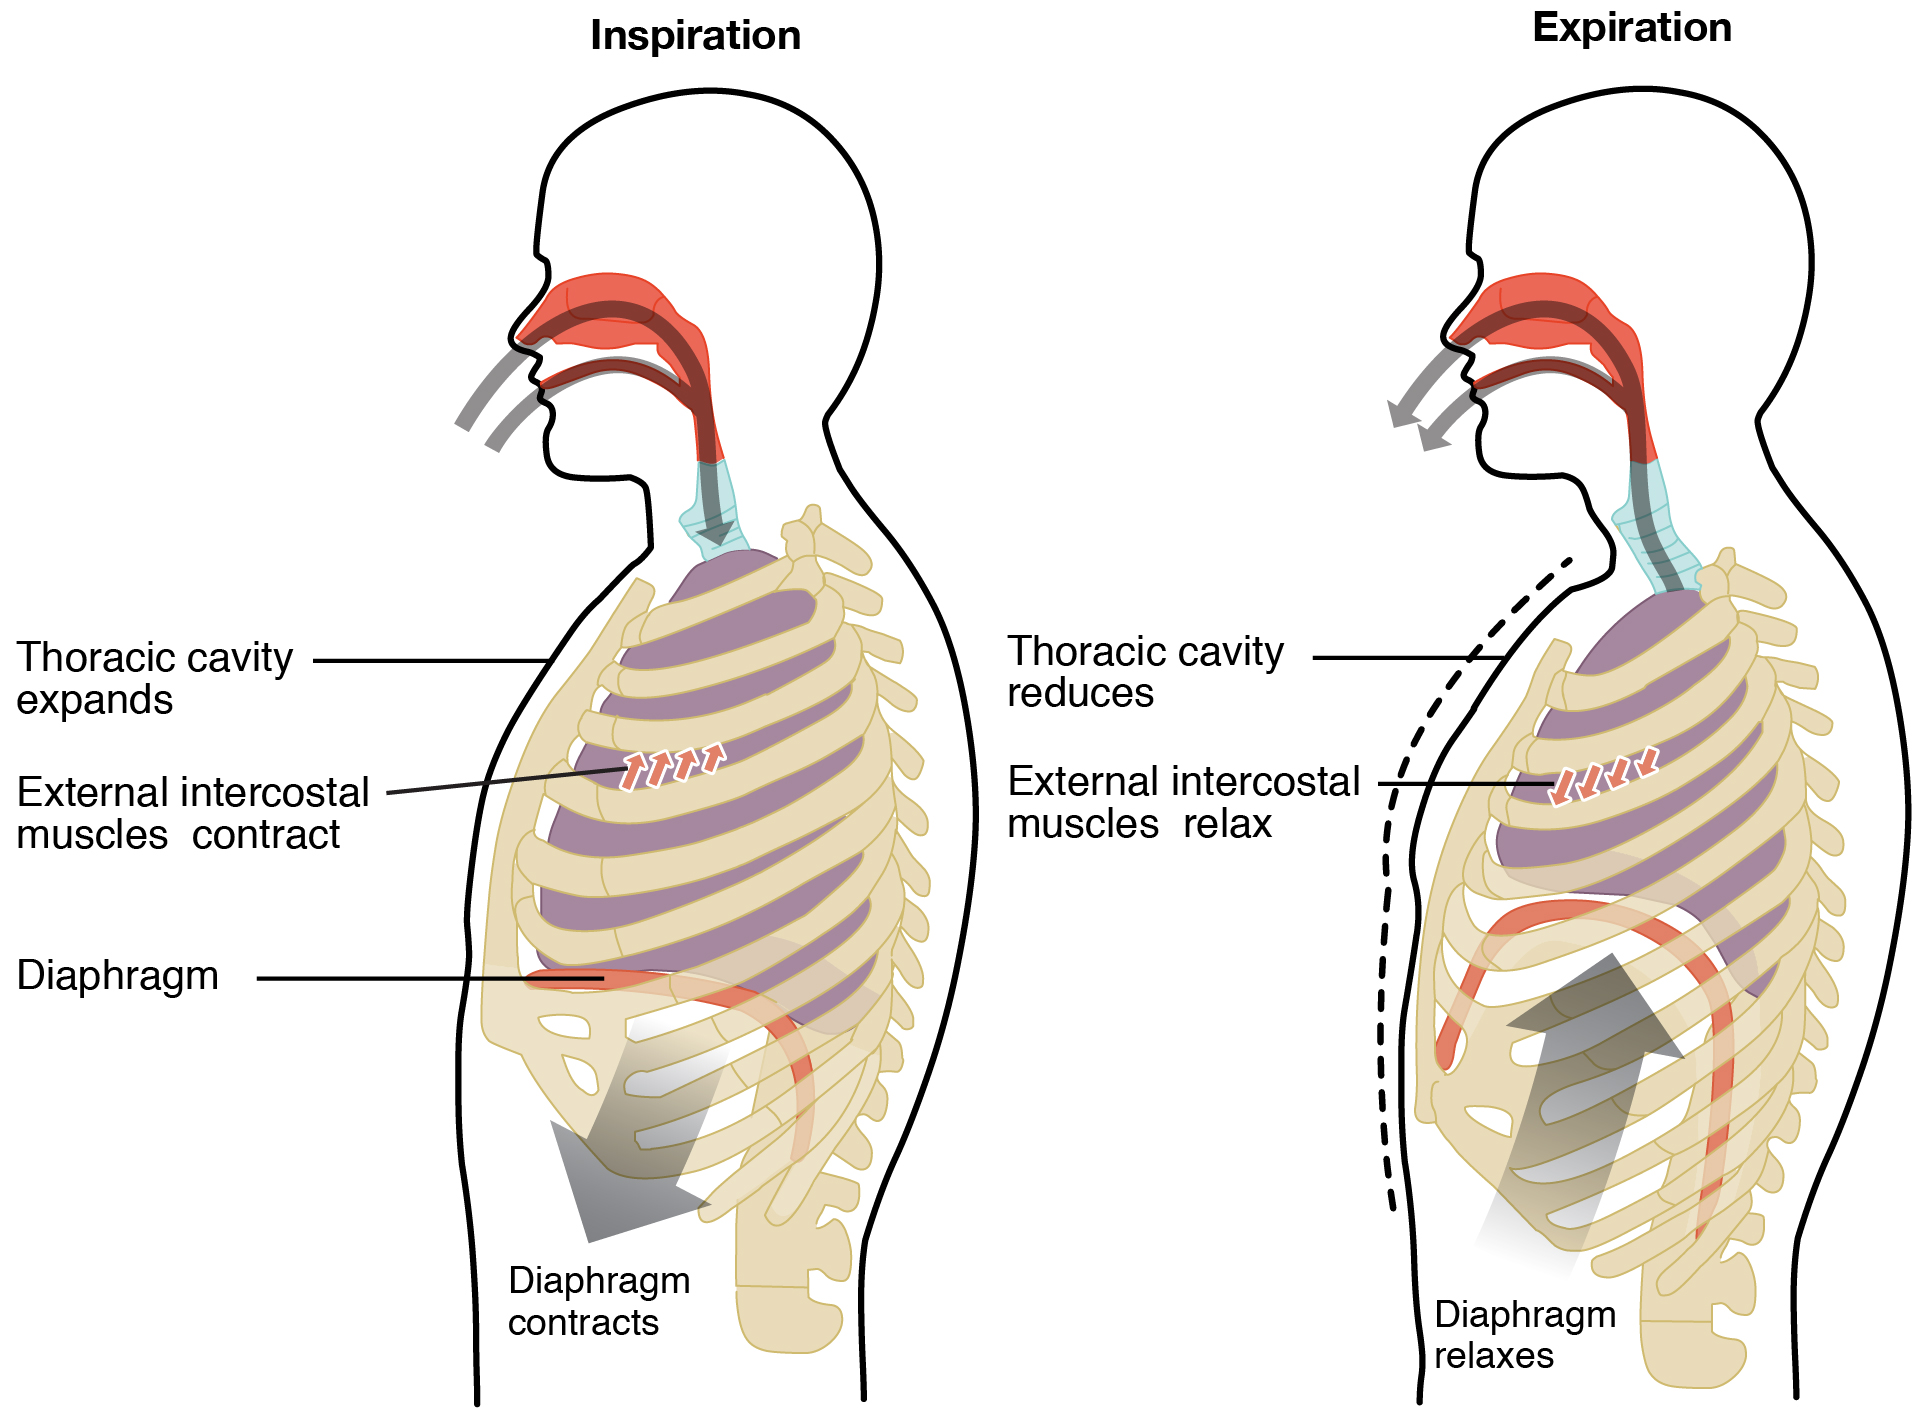
\includegraphics[width=.78\textwidth]{figures/intro_breathing_mechanics.png}\caption{Diagram of Respiration. Source: \href{https://commons.wikimedia.org/wiki/File:2316_Inspiration_and_Expiration.jpg}{OpenStax College}, \href{https://creativecommons.org/licenses/by/3.0/}{CC BY 3.0}; image content unchanged.}\label{fig:intro_breathing}\end{figure}
\FloatBarrier

Respiratory monitoring encompasses not only the frequency but also the rhythmic pattern of the breaths through time.  Waveform analysis of breathing automatically allows for transformation of a recording into a series of respiratory rates and identification of periods for more careful analysis \citep{charlton2018}.

The process of breathing is either registered directly using the airflow of the nose and mouth or by recording chest movements via a belt. The processes of breathing and expiration translate to waveforms. This raises another question: do other continuous physiological body measurements have waveforms that correspond to breathing rhythms?

\subsection{Why ECG?}
The electrocardiogram (ECG) is a graphical representation of voltage measured from electrodes on the skin that pick up the electrical activity of the heart. Every heart beat produces a wave form that looks almost identical, thus allowing one to determine its time. Figure~\ref{fig:intro_ecg} depicts an example of an idealized heart beat.
\begin{figure}[!htbp]\centering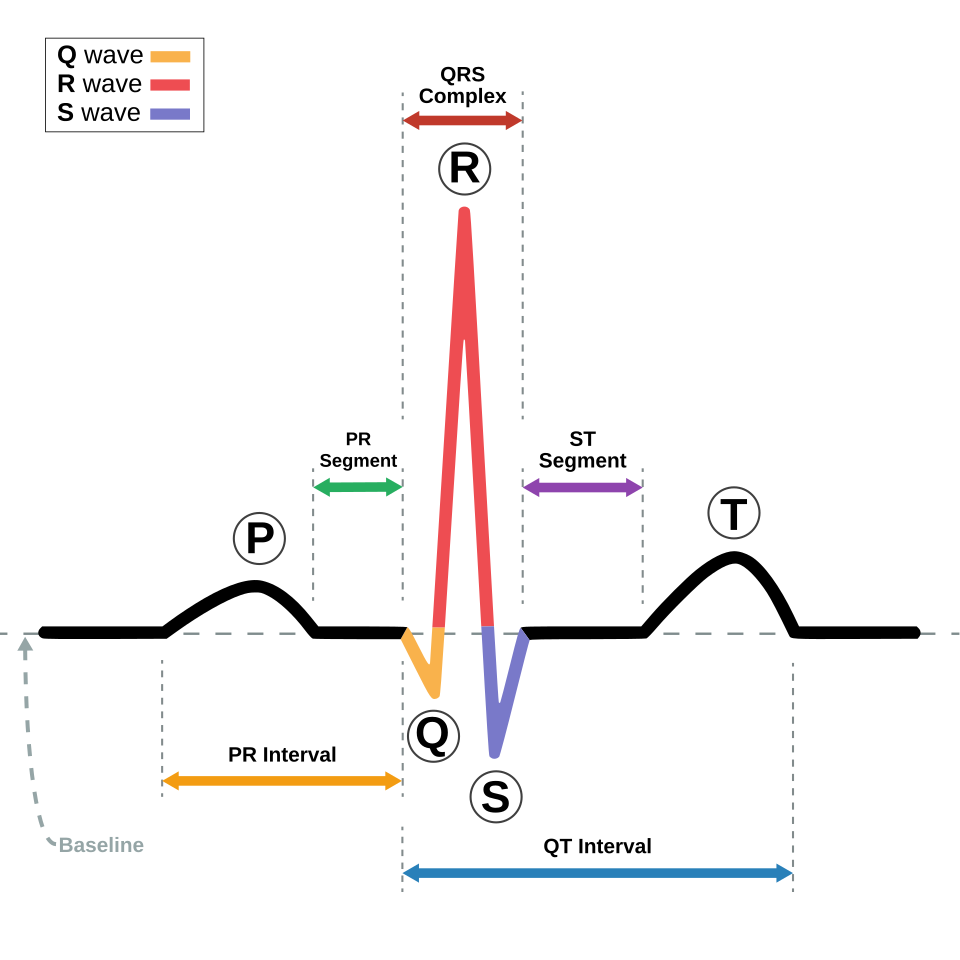
\includegraphics[width=.48\textwidth]{figures/intro_ecg_waveform.png}\caption{A schematic ECG waveform.Source: \href{https://commons.wikimedia.org/wiki/File:SinusRhythmLabels.svg}{Anthony Atkielski; SVG conversion by atom}, public domain; image content unchanged.}\label{fig:intro_ecg}\end{figure}
\FloatBarrier

When times of subsequent beats have been determined, one can find the difference in time between them. This difference is the R-R interval. The shorter the R-R interval, the higher the frequency of beats, while the longer the R-R interval is, the lower the frequency is.

\subsection{Why heartbeat changes can reveal breathing rhythm}
The act of breathing modifies the pressures on the chest cavity and the neurocontrol of the cardiac cycle. Breathing-induced heart rate variations are common and consist of an increase in heart rate during inspiration and a decrease during expiration. Correspondingly, the R--R intervals decrease and increase. This cyclical pattern is known as respiratory sinus arrhythmia \citep{charlton2018}. Hirsch and Bishop investigated the effect of breathing frequency and depth on these heart rate variations in humans, providing a physiological basis for estimating the breathing pattern from R-R intervals \citep{hirsch}.

Figure~\ref{fig:breathing_heartbeat} visualises this relationship using idealised curves. Breathing consists of an increase and decrease in heart rate, and the R--R interval curve follows the reverse path. The repetition time of these lower frequency oscillations gives an indicator to the breathing period. ECG-based respiration estimation thus starts with variations between successive heartbeats.

\begin{figure}[!htbp]\centering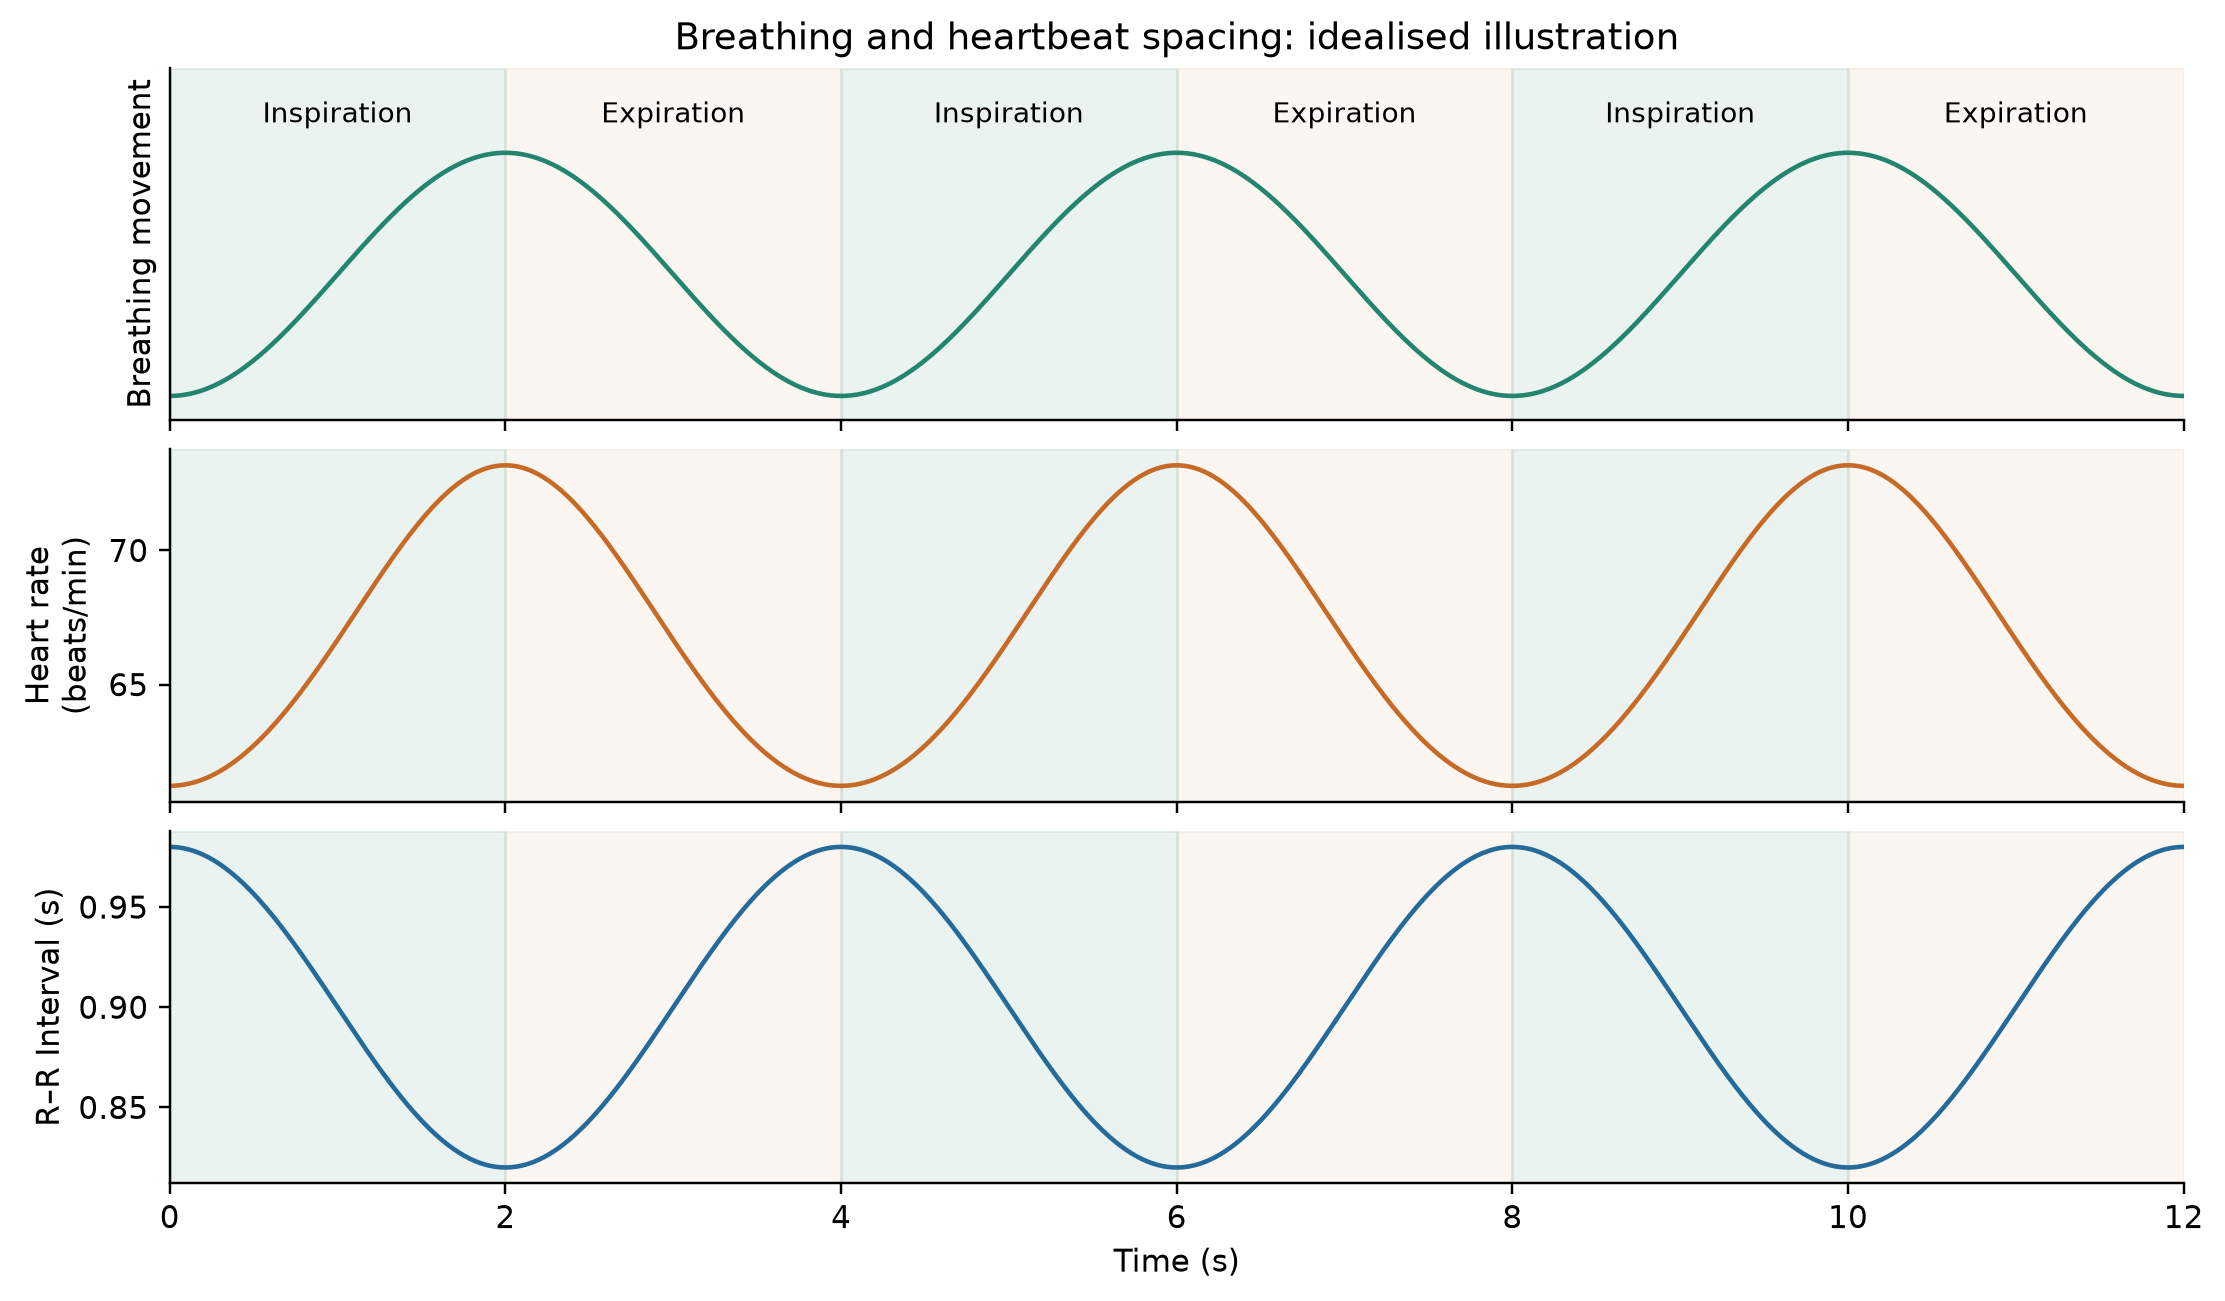
\includegraphics[width=.96\textwidth]{figures/explain_breathing_heartbeat.png}\caption{Idealised relationship between breathing, heart rate and R--R interval.}\label{fig:breathing_heartbeat}\end{figure}
\FloatBarrier

The movement of breathing will also influence the location of the heart concerning the electrodes, ECG height and local voltage. This information complements R-R interval measurements \citep{charlton2018}. The work is guided by the methodology of Peter H. Charlton et al. In 2016, Charlton, Timothy Bonnici, Lionel Tarassenko et al. systematically compared respiration-rate techniques based on ECG and pulse waves: extract information, estimate rates and then combine them \citep{charlton2016}. The 2018 review by Charlton et al. further structured physiological grounds and steps of the algorithm \citep{charlton2018}.

This report will do the same: find ECG measurements which can depend on breathing, construct the corresponding curves that can be counted in cycles and compare the results with chest registration at the same time. 
\newpage
\section{Build a respiratory pipeline using supplied QRS}
The first run uses heartbeat markers distributed with the data. This chapter explains each step and the sources of its settings; Chapter 3 then compares the baseline output with the chest-derived reference respiratory rate.

\begin{figure}[!htbp]\centering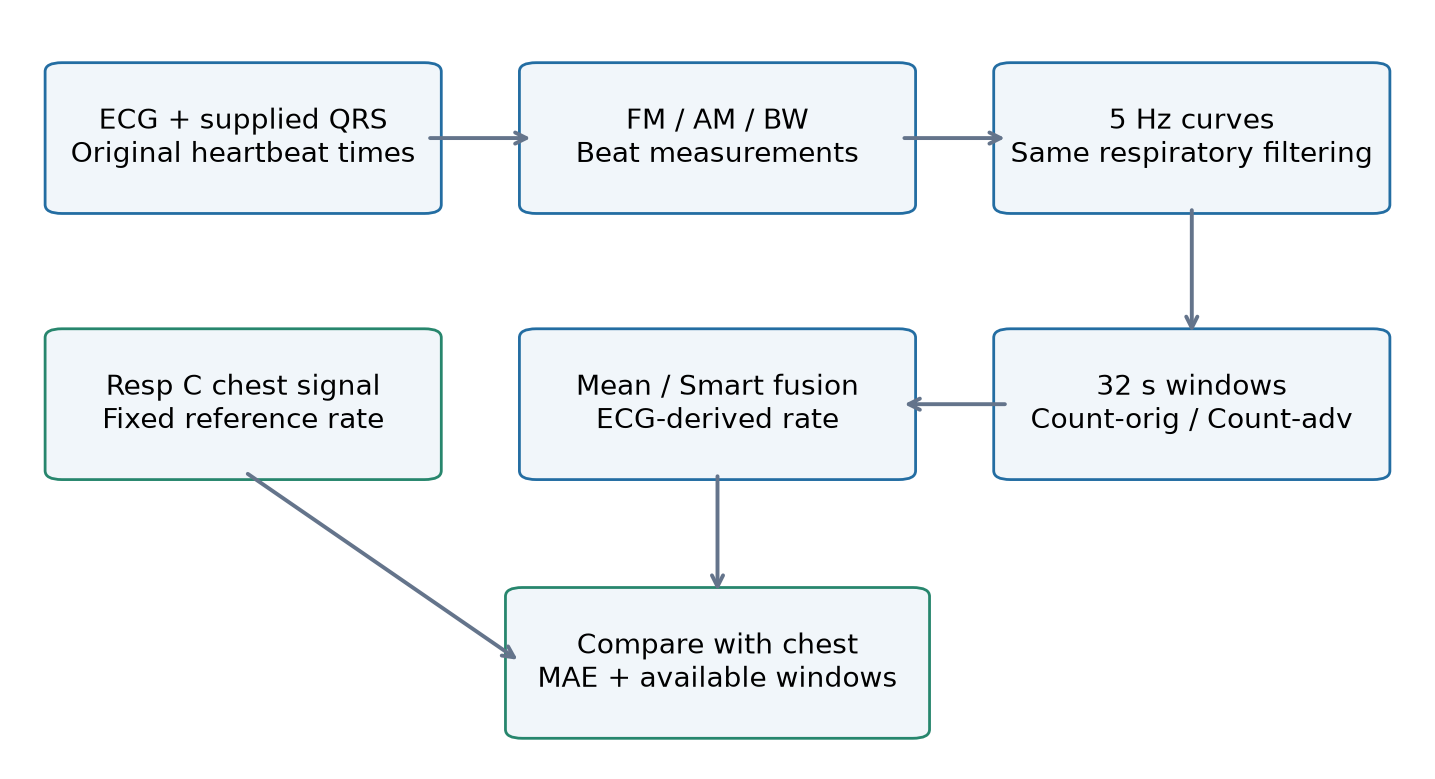
\includegraphics[width=.96\textwidth]{figures/supplied_pipeline.png}\caption{The first run uses supplied QRS only.}\label{fig:baseline_pipeline}\end{figure}
\FloatBarrier
\subsection{Input recordings and heartbeat times}
In Apnea-ECG, files a01--a04, b01 and c01--c03 include both ECG and respiratory signals \citep{penzel,goldberger}. ECG signal provides the estimate, while the chest recording makes it possible to compare its rhythm with separately recorded breathing signal. It is the pairing of the signals that defines the sample. Complete recordings include regular periods, noisy periods and transitions during the night.

For analysis, we use the chest channel called Resp C. The baseline uses the supplied QRS markers; for the next run, we keep the same chest recording. Information about minute-level apnoea labels is used as the background information, while cycle level timing is obtained from the chest signal.

Both ECG and chest signals have 100 samples per second (100 Hz) \citep{penzel}. ECG values are normalized to millivolts for visual analysis and the measure of amplitudes. Time period of interest covers the time period for both signals, so we get 7,431 32 second segments (from Charlton et al., 2016, section 3.5 \citep{charlton2016}) (see Table~\ref{tab:inventory}).Results are examined by recording before they are pooled.

\begin{table}[!htbp]\centering\small\begin{tabular}{lrrrr}
\toprule
Record & ECG samples & Resp samples & Duration (s) & $N$ \\
\midrule
a01 & 2957000 & 2956796 & 29567.96 & 923 \\
a02 & 3182000 & 3181796 & 31817.96 & 994 \\
a03 & 3135000 & 3134796 & 31347.96 & 979 \\
a04 & 2980000 & 2979796 & 29797.96 & 931 \\
b01 & 2917000 & 2916796 & 29167.96 & 911 \\
c01 & 2899000 & 2898796 & 28987.96 & 905 \\
c02 & 3007000 & 3006796 & 30067.96 & 939 \\
c03 & 2720000 & 2719796 & 27197.96 & 849 \\
\bottomrule
\end{tabular}
\caption{Selected recordings.}\label{tab:inventory}\end{table}
\FloatBarrier

Transforming the schematic representation into a real-time recording entails the process of converting the continuous wave into the series of time instances when heartbeats occurred.
In the figure a01, you can see the repeated QRS waves used to define the locations of heartbeats one after another.
The time interval between two adjacent heartbeats is called the R-R interval. If the intervals are smaller, then the heart rate is higher; and vice versa. For the interval expressed in seconds, the number of beats per minute can be calculated as $60/\text{interval}$.
\begin{figure}[!htbp]\centering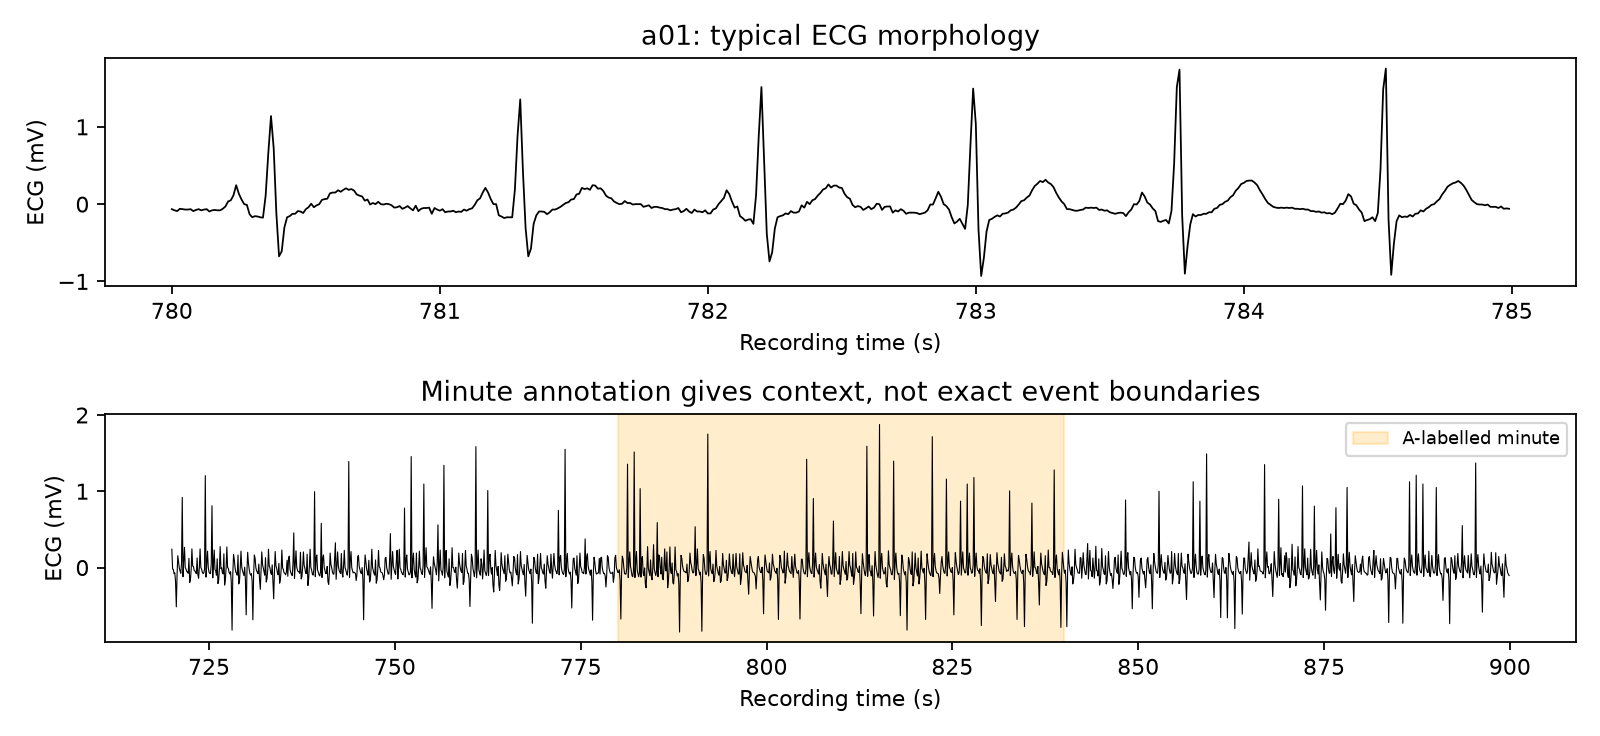
\includegraphics[width=.96\textwidth]{figures/assignment_waveforms.png}\caption{Scaled ECG morphology and a minute-level A annotation in a01.}\end{figure}
\FloatBarrier

\subsection{FM, AM and BW}

\begin{figure}[!htbp]\centering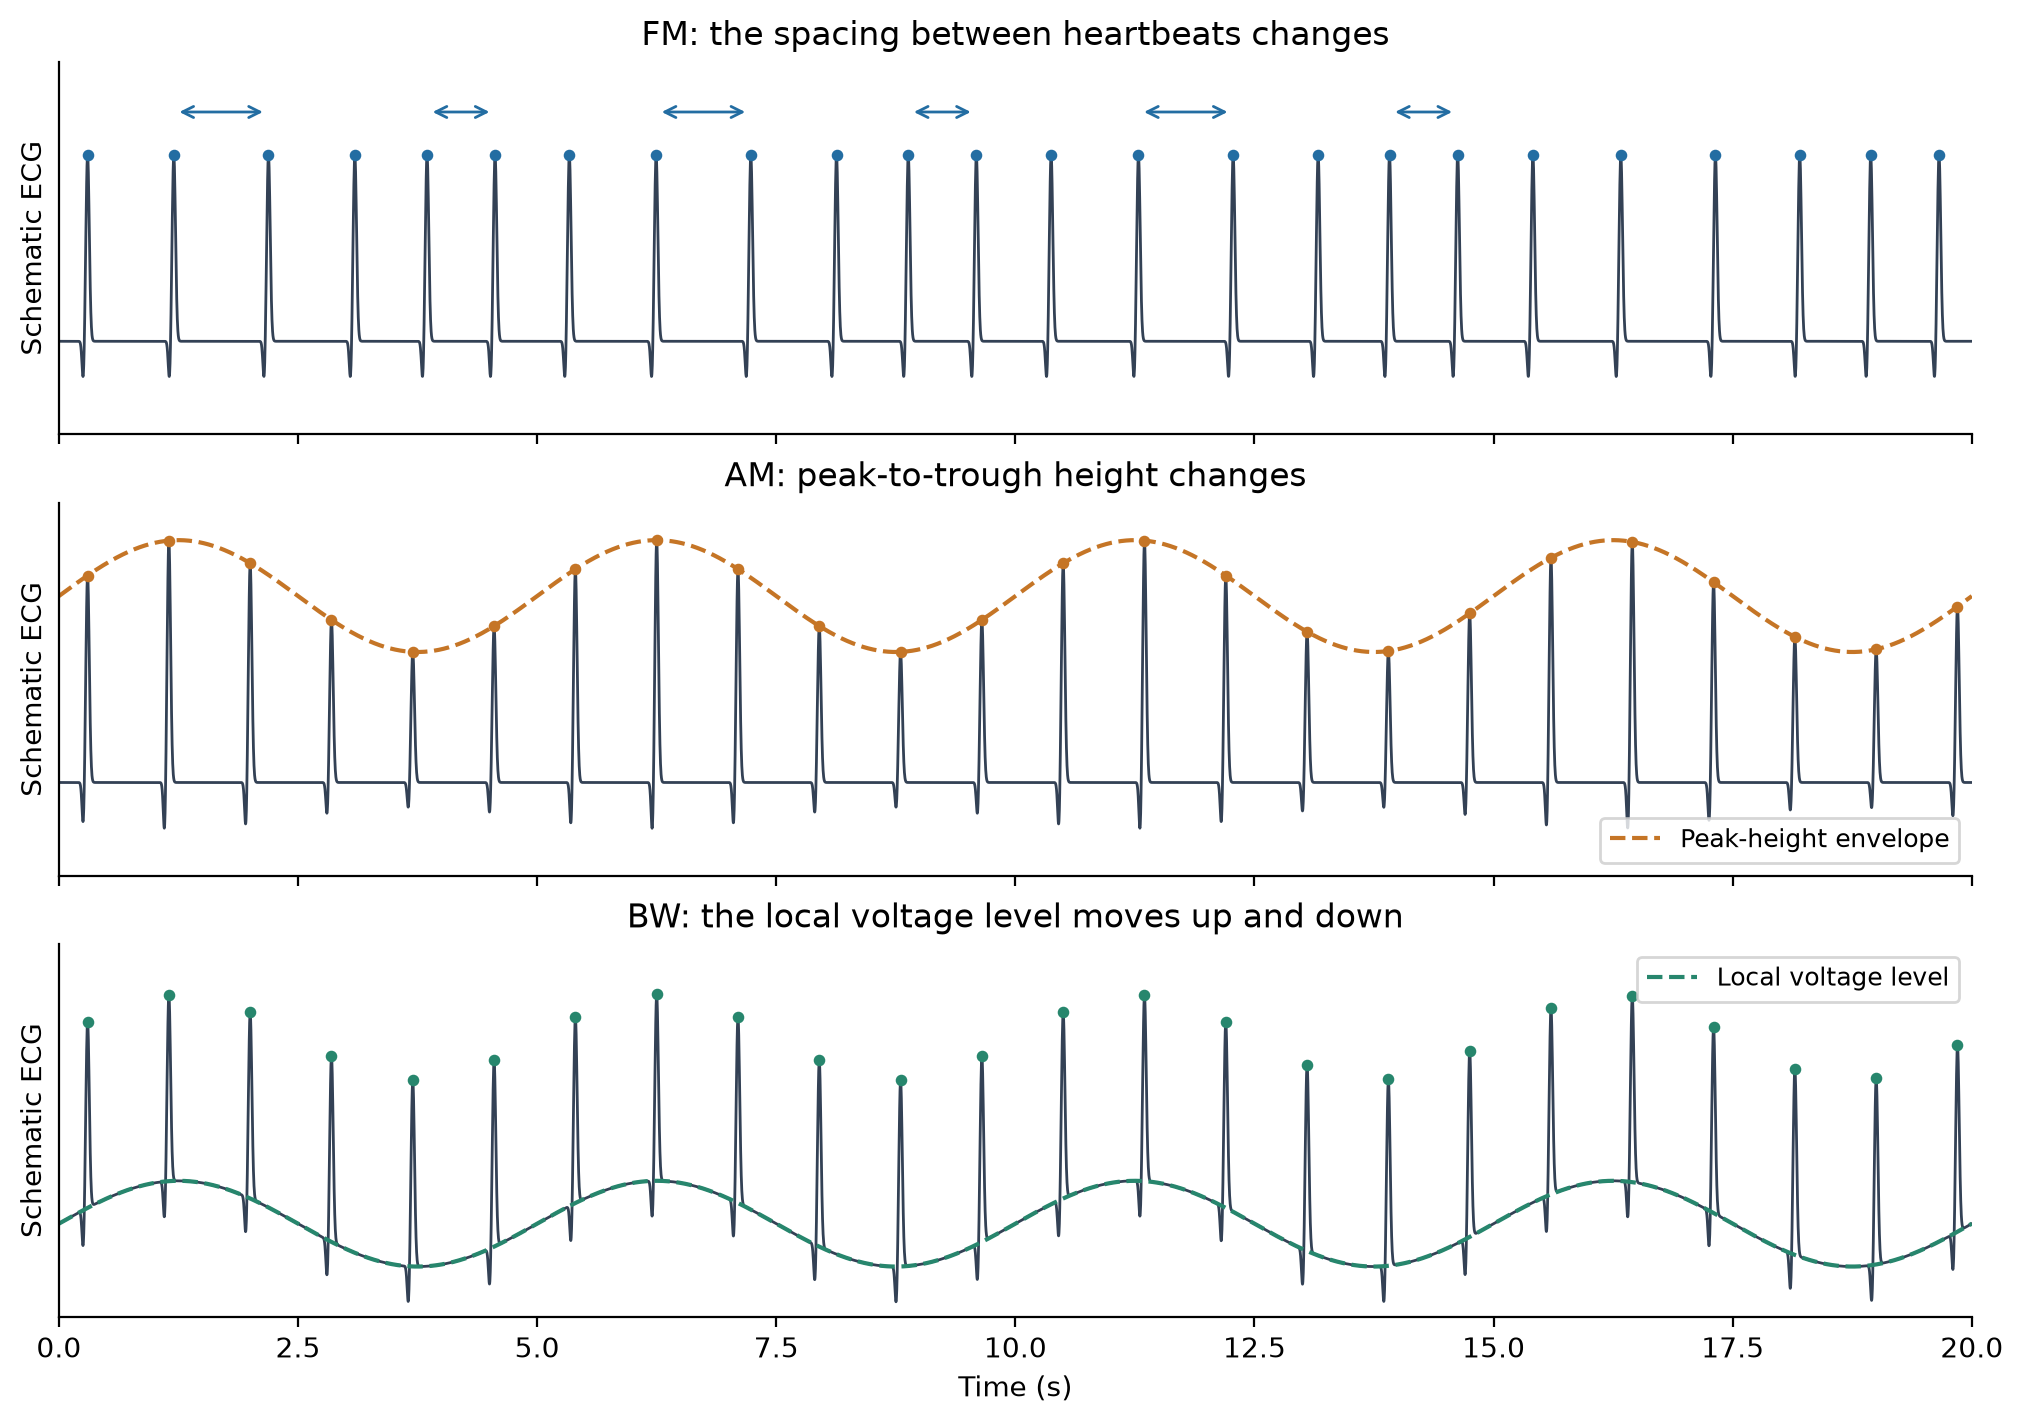
\includegraphics[width=.96\textwidth]{figures/three_respiratory_clues.png}\caption{Three isolated respiratory clues in constructed ECG signals: changing heartbeat spacing (FM), amplitude (AM) and local voltage level (BW).}\label{fig:three_clues}\end{figure}
\FloatBarrier
The \textbf{interval clue (FM)} represents the time duration between successive beats. If $b_i,b_{i+1}$ are two samples of beats and $f_s$ is the sampling frequency, then the interval $I_i=(b_{i+1}-b_i)/f_s$ is located halfway between the two beats and is scaled by the mean interval of the entire record:
\begin{equation}
F_i=I_i/\overline I.
\end{equation}
In the case $\overline{I}$ refers to the mean interval. Normalizing by the full record mean and choosing interval midpoints are choices made in the project to ensure consistency of the presentation with respect to oscillations timing.

The \textbf{amplitude clue (AM)} refers to the height between a local peak and a trough. The \textbf{baseline clue (BW)} refers to their mean voltage value. They adhere to common features for estimating respiration from ECG \citep{charlton2016}. The previous trough selection criterion of 0.1 s before follows \citet{charlton2016}, section 2.1. The peak selection criterion up to 0.2 s after a marker follows the companion toolbox \citep{charlton2016}. This provides amplitude estimation at local peaks and troughs. Once a peak is chosen several times, it is considered only once. The current amplitude selection procedure does not alter the heartbeat times for FM.

For peak voltage $p_i$, trough voltage $q_i$ and full-record mean peak-trough difference $D=\operatorname{mean}(p_i-q_i)$,
\begin{equation}
A_i=(p_i-q_i)/D,\qquad B_i=(p_i+q_i)/(2D).
\end{equation}
The difference describes waveform height; the average describes its local voltage level. Both are divided by the same fixed scale $D$ to show relative changes over time.

\begin{figure}[!htbp]\centering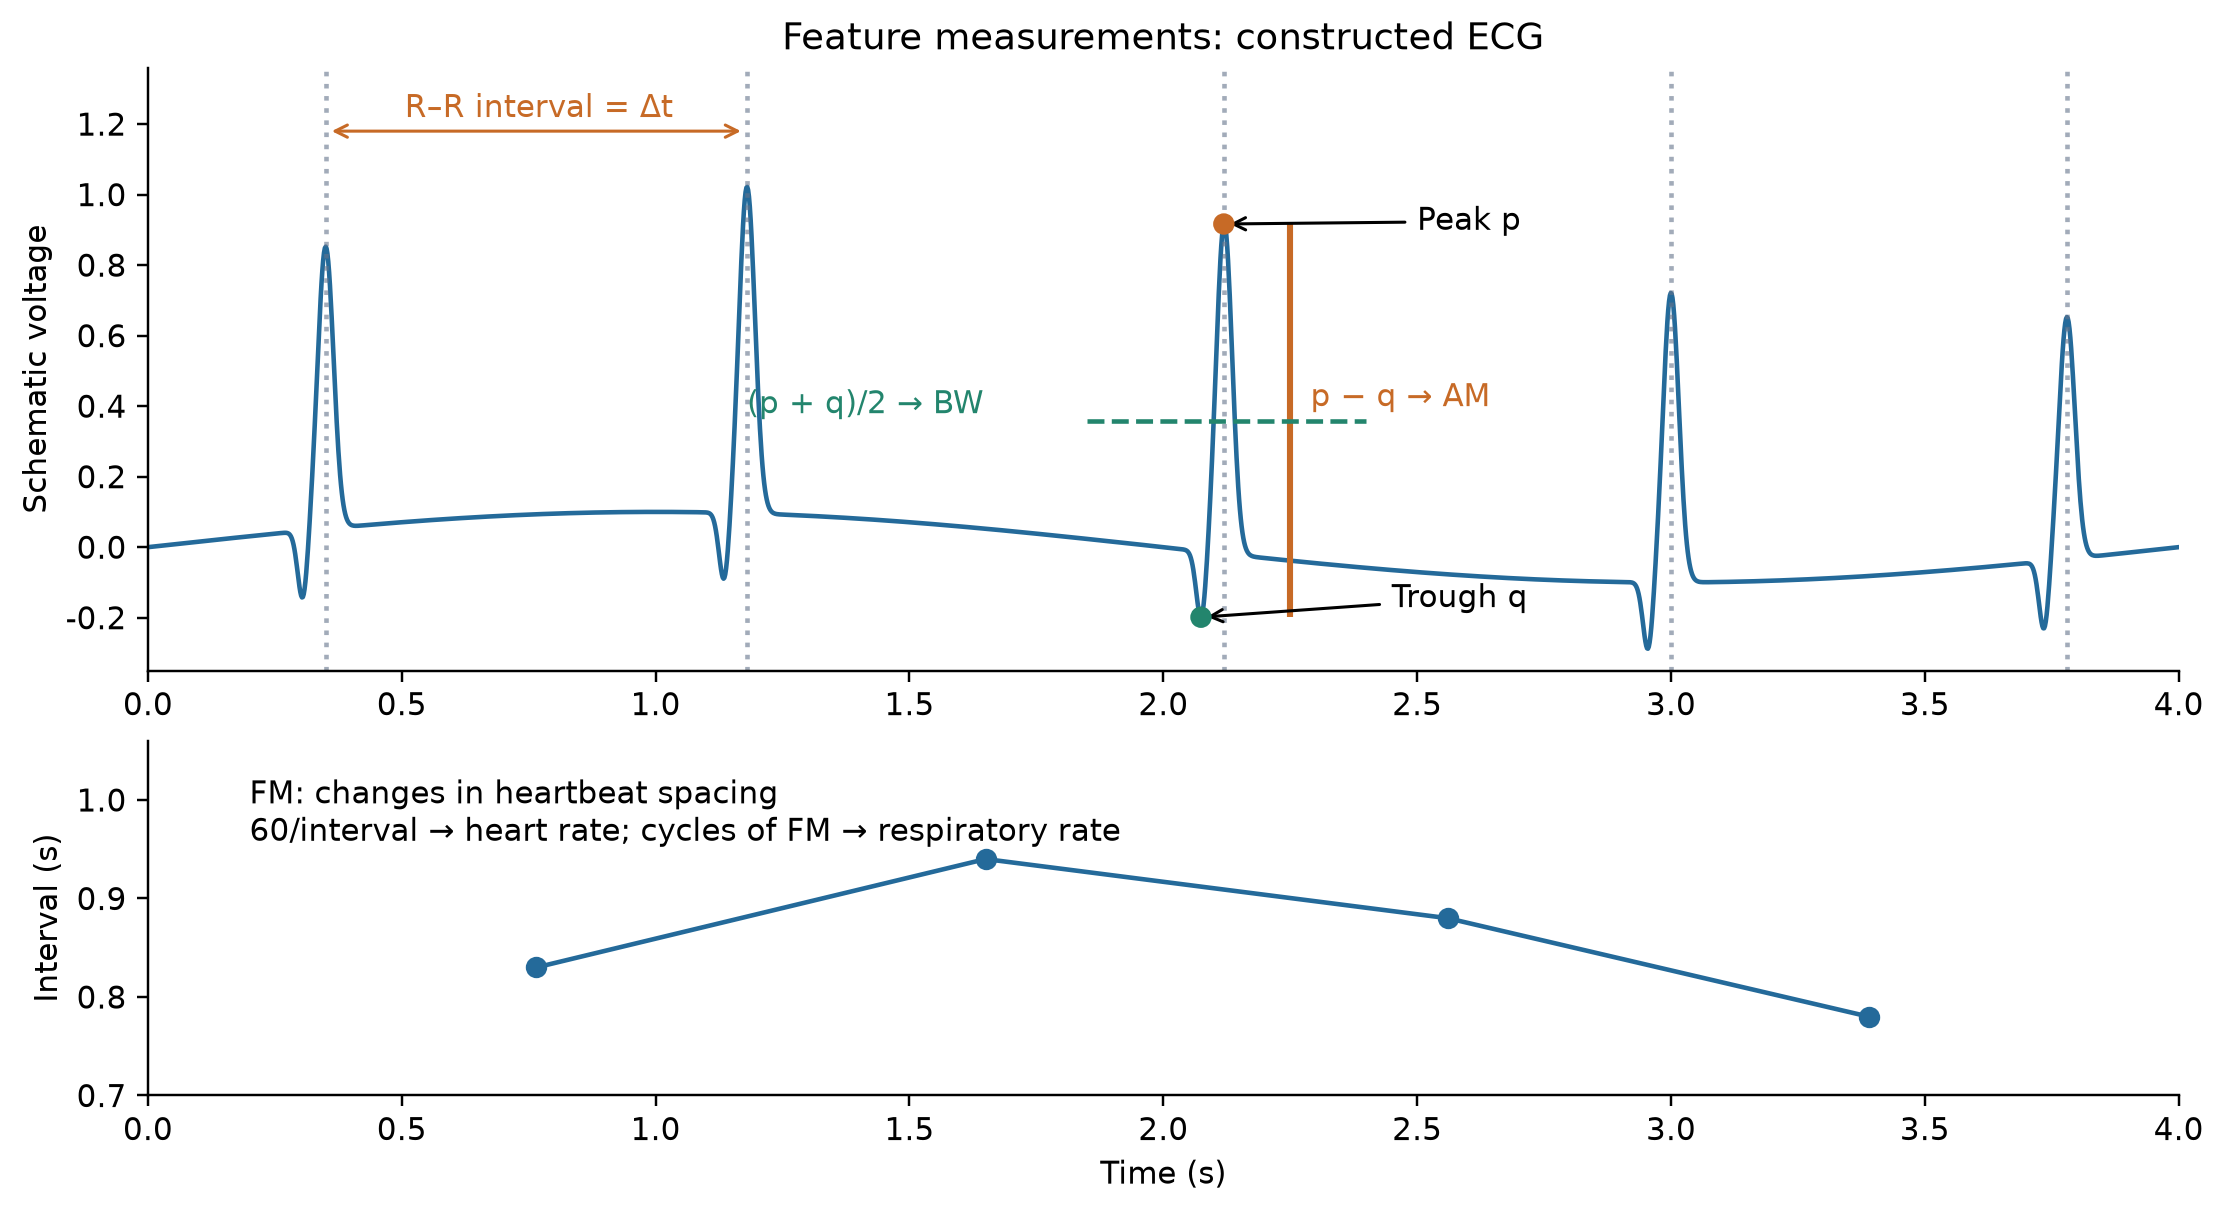
\includegraphics[width=.96\textwidth]{figures/explain_features.png}\caption{Definition sketch for R--R, AM and BW.}\label{fig:features}\end{figure}
\FloatBarrier

\subsection{Prepare curves whose cycles can be counted}
The heartbeat measurements come irregularly in time. We link adjacent measurements to construct five-point-per-second curves, as per Charlton et al., section 2.1 \citep{charlton2016}. Links are made only between existing data points. Over a long interval of time, the linking line will be dependent on scant data at its extremities.

After removing the general linear trend and minimizing slow drift and fast fluctuations, the respiratory variation becomes easier to count. Processing the entire curve first and then dividing it into segments results in less effect of repeated processing of edges of short segments. All the two heartbeat sources go through exactly the same processing procedure. Figure~\ref{fig:processing} illustrates the comparison of the original beat measurement, the linked curve, and the processed curve in a real segment.
Figure~\ref{fig:processing}: In Figure~\ref{fig:processing}, each orange dot represents one heartbeat measurement. The central graph connects adjacent measurements using straight lines and samples at every 0.2 s on the stated 5 Hz grid. The bottom graph is cropped after full-record processing. Cycle counting is done after this step.

\begin{figure}[!htbp]\centering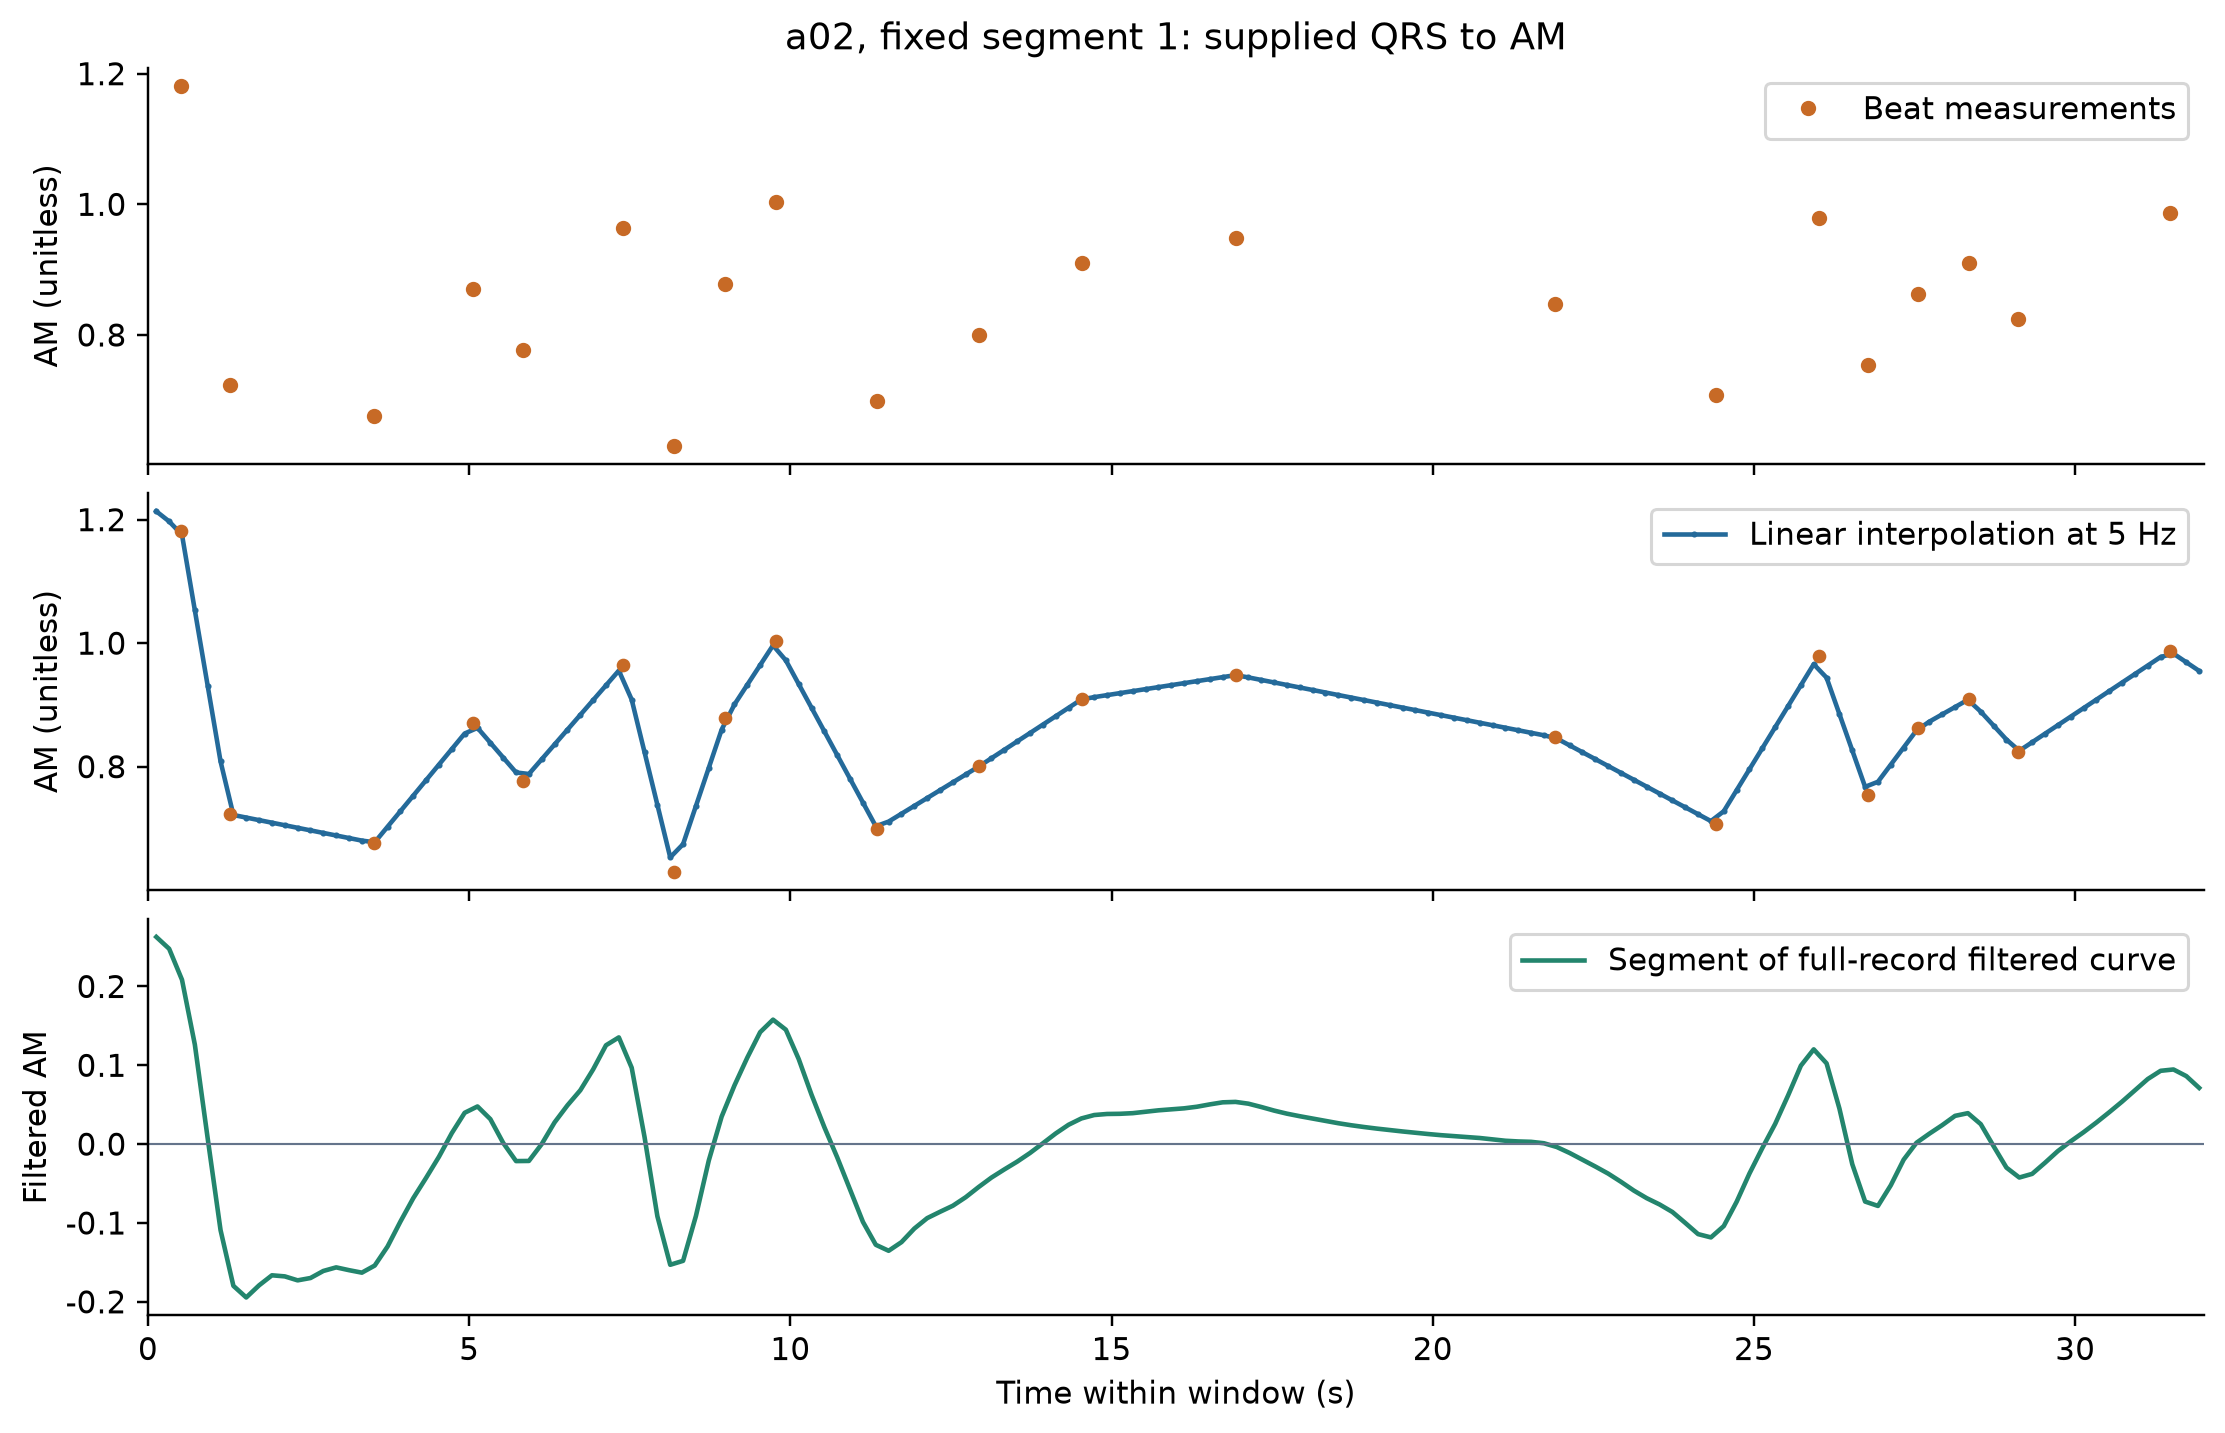
\includegraphics[width=.96\textwidth]{figures/baseline_processing.png}\caption{AM processing in one real segment.}\label{fig:processing}\end{figure}
\FloatBarrier

\subsection{Count cycles within 32 s segments}
The length should be sufficient to provide a reliable average rate but not too long to reflect local variations. 32 s length by Charlton et al. (2016), section 3.5 \citep{charlton2016} is used. For instance, constant breathing with 15 breaths/min will yield eight cycles in 32 s. A segment starts at zero recording time and never overlaps with others. Partially filled final segment is discarded from consideration.

For each clue, two cycle-counting methods are applied \citep{charlton2016}. \textbf{Count-orig} algorithm consists in creation of cycles by means of peaks and troughs, calculation of average duration of valid cycles and conversion to cycles per minute. \textbf{Count-adv} algorithm eliminates local perturbations first and then computes the rate based on complete cycles and their duration. The algorithms are different in what oscillations are considered and, therefore, one and the same graph can yield different rates (Figure~\ref{fig:counters}).


\begin{figure}[!htbp]\centering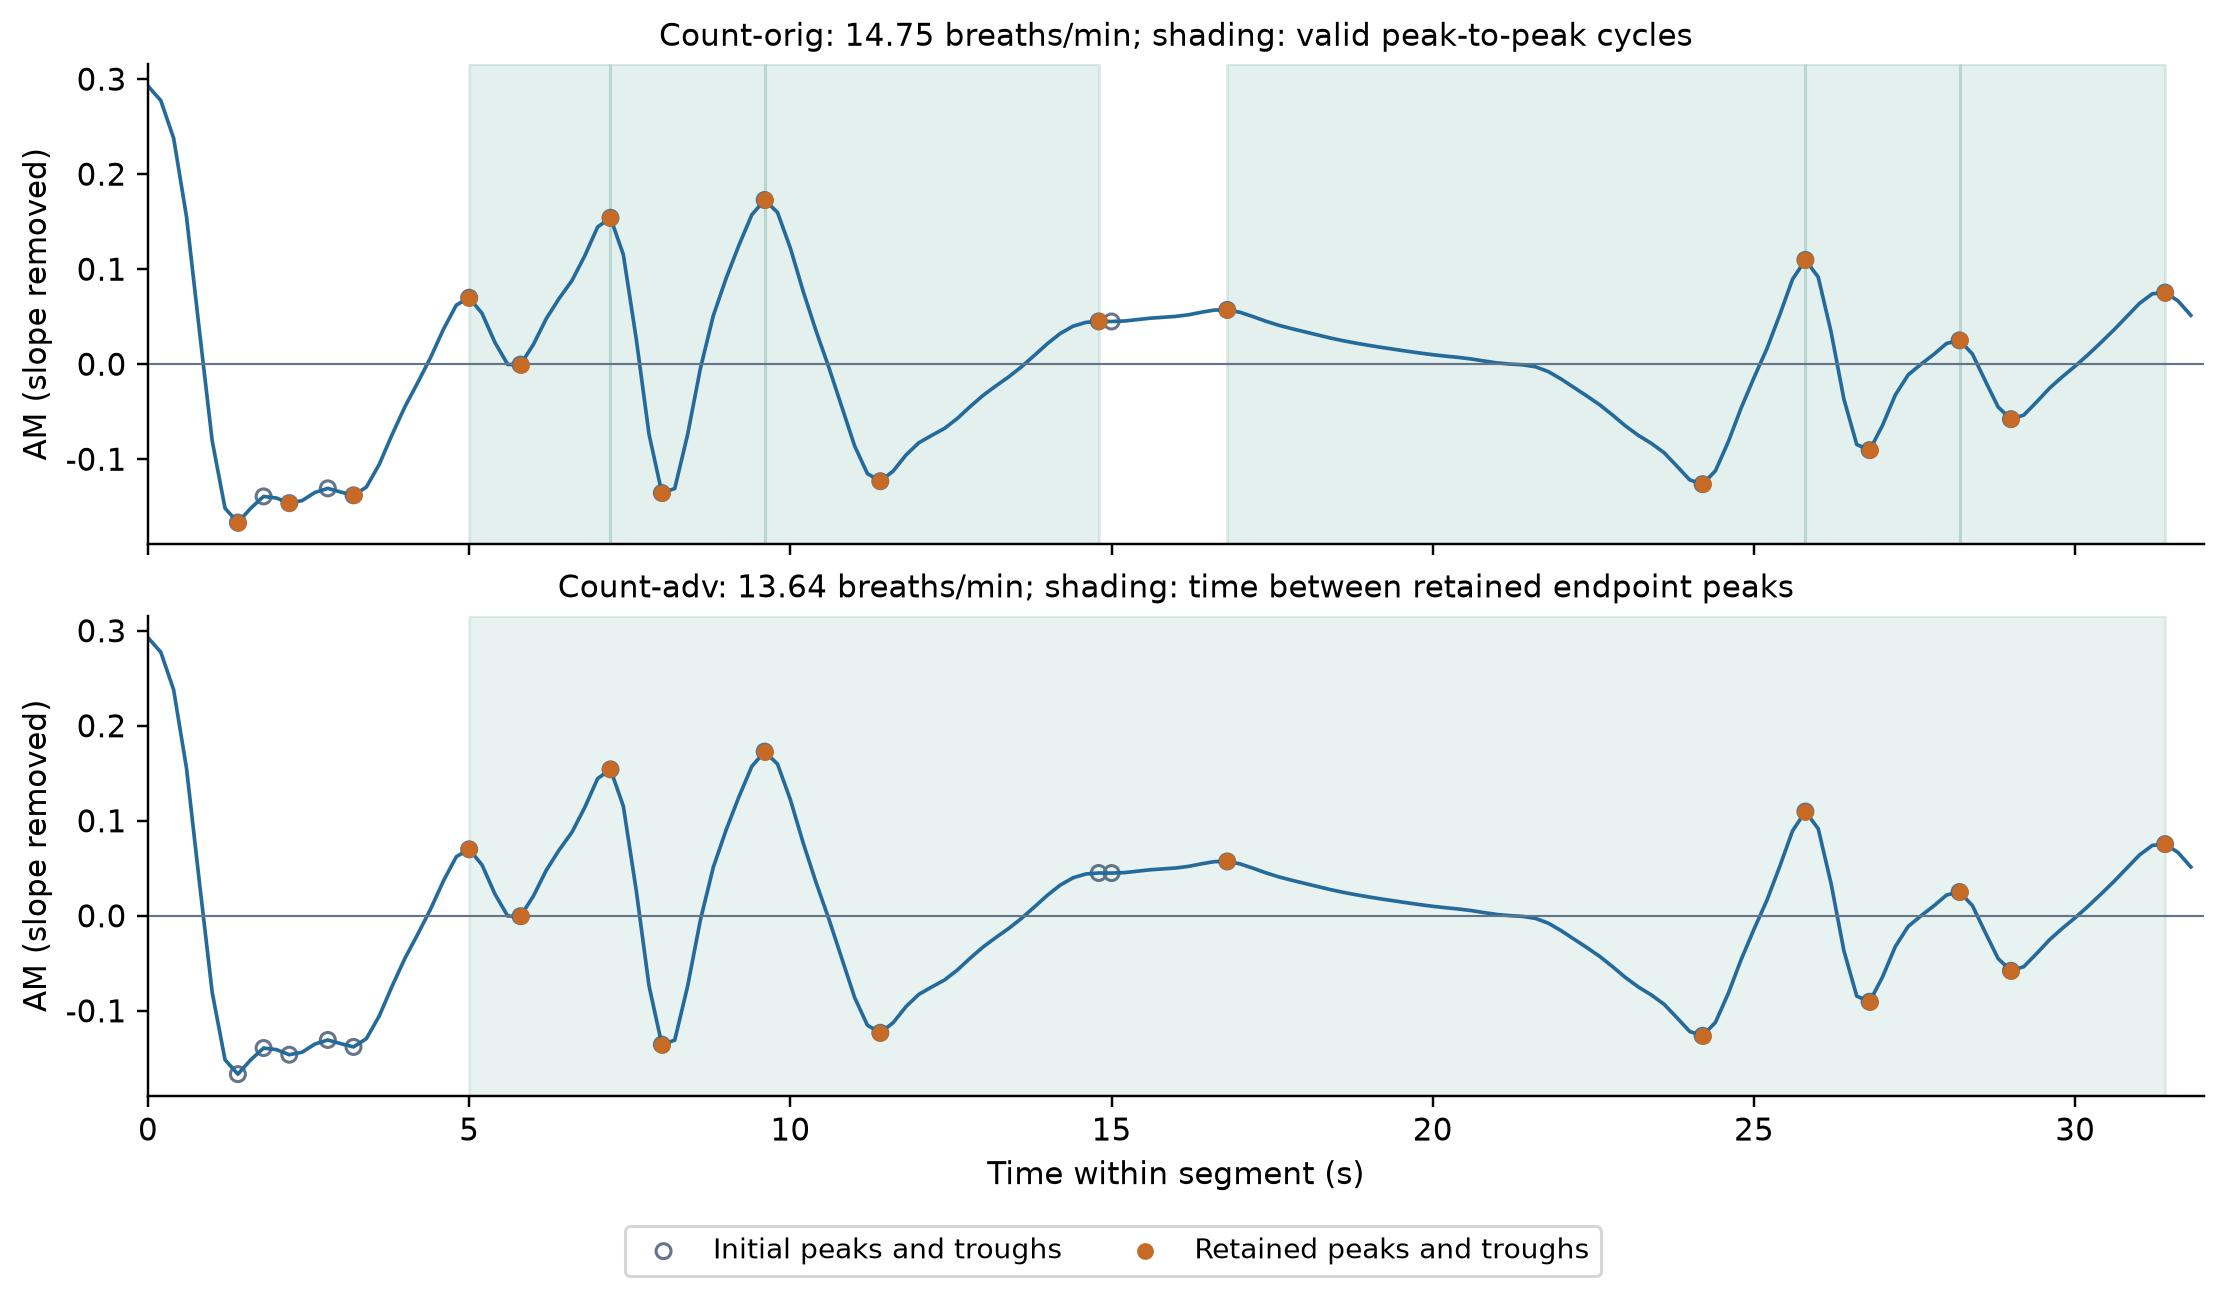
\includegraphics[width=.96\textwidth]{figures/baseline_counters.png}\caption{Different cycle rules on the same real supplied-QRS feature}\label{fig:counters}\end{figure}
\FloatBarrier

\subsection{Combine three estimates into one rate}
Each clue yields a respiratory rate. The first combination uses their direct mean; each clue counts equally and requires all three rates. The second combination, \textbf{Smart fusion}, determines whether the rates are close enough to accept the mean \citep{charlton2016}.

For individual rates $r_F,r_A,r_B$, the mean is $\overline r=(r_F+r_A+r_B)/3$. Their dispersion is measured by the standard deviation $s$, with acceptance condition
\begin{equation}
s=\sqrt{\frac{(r_F-\overline r)^2+(r_A-\overline r)^2+(r_B-\overline r)^2}{2}}\le4\ \bpm.
\end{equation}
A smaller standard deviation implies proximity between the individual rates. An acceptable estimate using Smart fusion is the same as the direct mean; however, a dispersion exceeding 4 breaths/min results in no estimate at all. The limit stems from Charlton et al. (2016), Table 3 \citep{charlton2016}. Figure~\ref{fig:fusion} displays an accepted and a rejected sample segment.

Four baseline settings use two cycle-counting methods and two fusion methods; the direct mean of equally weighted clues acts as the baseline for the project. In the future figures and tables, orig/adv refer to the two cycle-counting methods, while mean/smart stand for the direct mean and Smart fusion.
\begin{figure}[!htbp]\centering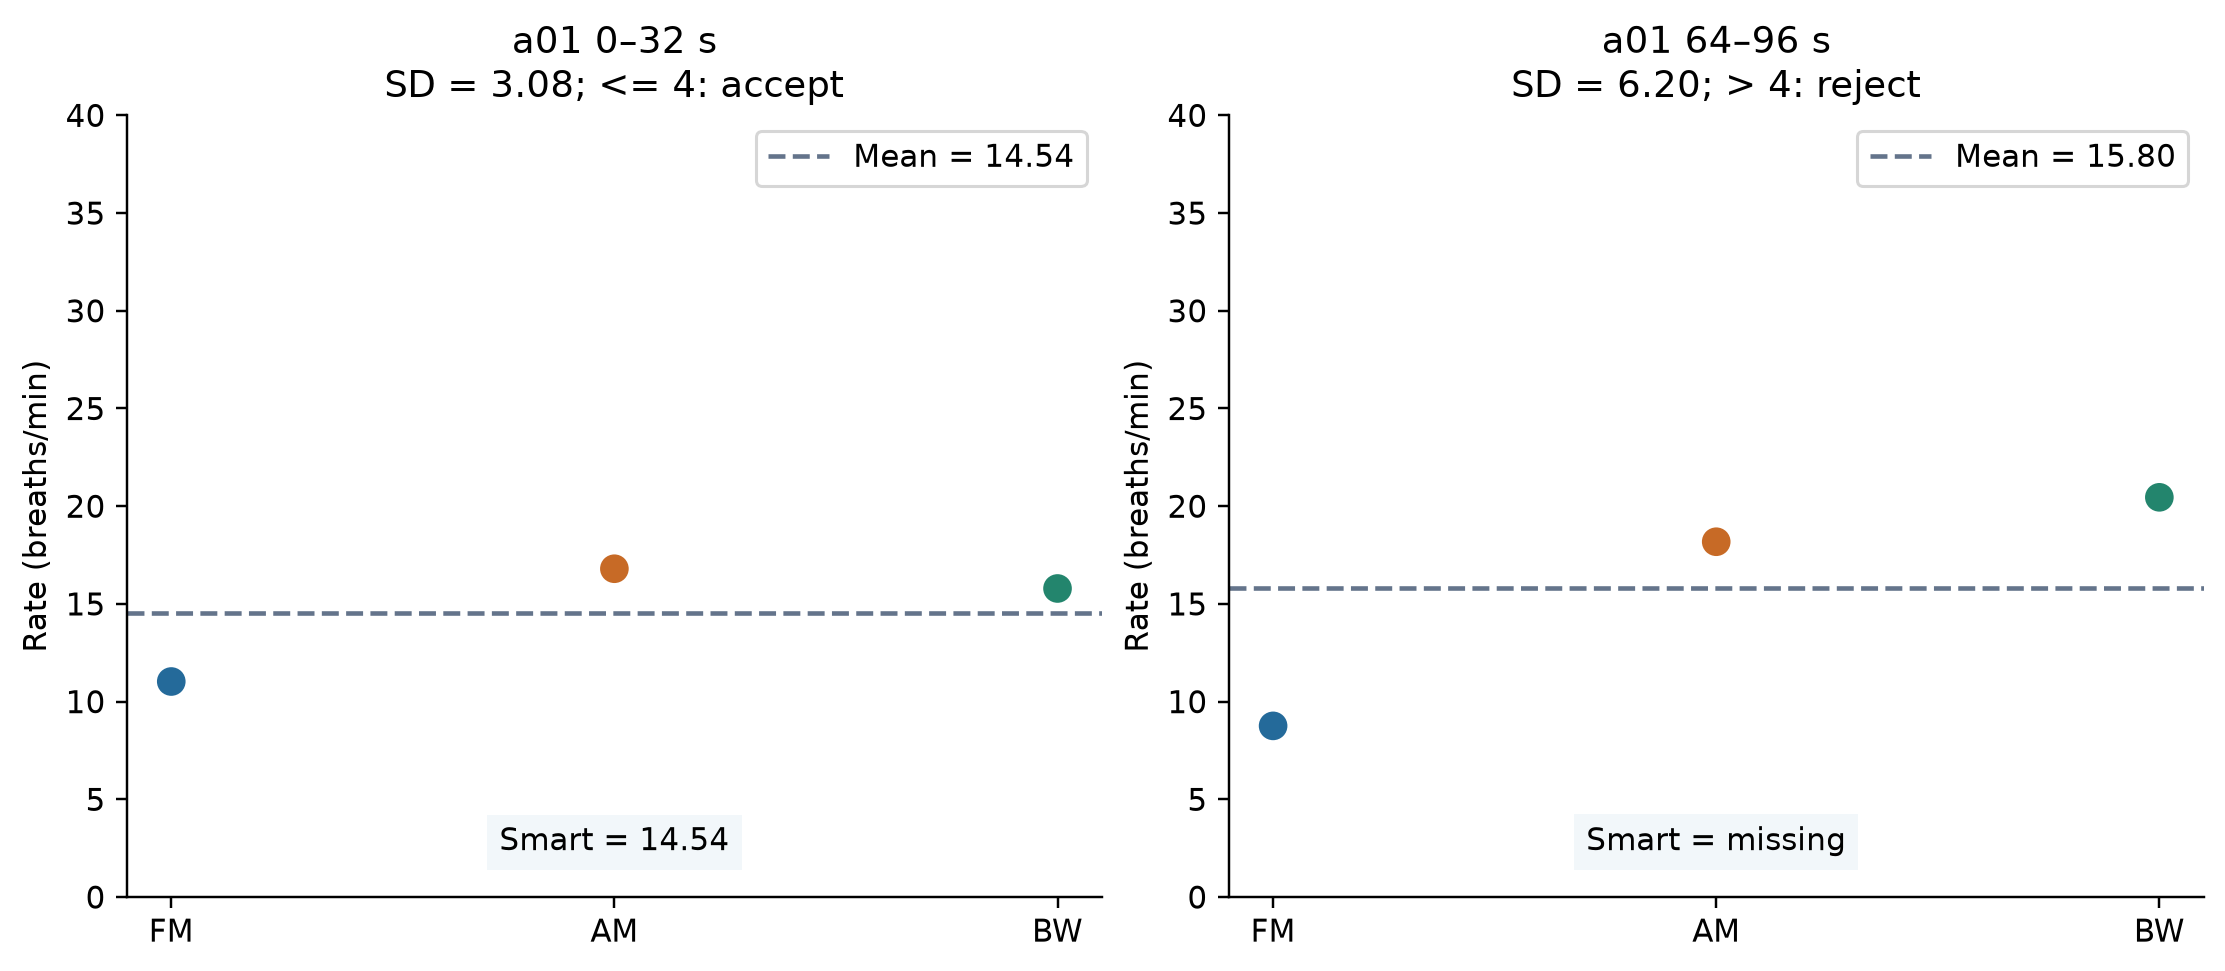
\includegraphics[width=.96\textwidth]{figures/baseline_fusion.png}\caption{Supplied-QRS/Count-adv individual rates in two real a01 scoring windows.}\label{fig:fusion}\end{figure}
\FloatBarrier

\subsection{chest-derived reference respiratory rate and comparison measures}
Resp C is down-sampled to 5 Hz，32 seconds interval and analyzed using the same respiratory feature module and Count-adv. 

Mean absolute error (MAE) quantifies the average deviation in breaths per minute; coverage quantifies the share of all candidates with the estimate and reference. Using $e_w=\hat r_w-r_w^C$, 
\begin{equation}
\operatorname{MAE}=|\mathcal P|^{-1}\sum_{w\in\mathcal P}|e_w|,\qquad
\operatorname{bias}=|\mathcal P|^{-1}\sum_{w\in\mathcal P}e_w.
\end{equation}
The following metrics quantify the average over/underestimation: Bias. Here $N$ is the number of all candidates; $R$ and $E$ are the number of available references and estimates; $P$ is the number of pairs. Coverage is $100P/N$. 

Also included in the project design is waveform analysis: splitting each record into five equal-time portions and examining the middle portion of that length, producing 40 fixed candidates. Time-based analysis is followed by the additional examples chosen among results, relating differences in rates to raw waveforms.

\FloatBarrier
\newpage

\section{Supplied-QRS results and analysis of discrepancies}
\subsection{Compare the baseline ECG estimates with chest respiration}
The first run follows Chapter 2 using only supplied QRS markers. Table~\ref{tab:baseline} gives four counter/combination settings. The chest-derived reference respiratory rate is available in 7,317 of 7,431 candidates. Count-adv with a direct mean gives MAE 3.412 breaths/min on 7,289 paired segments; Smart fusion gives 3.206 on 5,285. Count-orig gives 4.422 and 3.825 breaths/min for the two combination rules.

\begin{table}[!htbp]\centering\small\begin{tabular}{llrrr}\toprule Counter & Fusion & Paired windows & Coverage (\%) & MAE\\\midrule
adv & mean & 7,289 & 98.09 & 3.412\\
adv & smart & 5,285 & 71.12 & 3.206\\
orig & mean & 6,820 & 91.78 & 4.422\\
orig & smart & 4,776 & 64.27 & 3.825\\
\bottomrule\end{tabular}\caption{Supplied-QRS baseline outputs.}\label{tab:baseline}\end{table}

\subsection{Results for each record}
Per-record results locate the discrepancies (Table~\ref{tab:baseline_records}). In a02, Count-adv with the direct mean has MAE 5.699 breaths/min and bias $-3.747$ breaths/min, showing an overall tendency to underestimate the chest rate. Figure~\ref{fig:baseline_night} follows the estimates, chest-derived reference respiratory rate and errors throughout the night.

\begin{table}[!htbp]\centering\small\begin{tabular}{lrrr}\toprule Record & Paired windows & Coverage (\%) & MAE\\\midrule
a01 & 919 & 99.57 & 3.686\\
a02 & 982 & 98.79 & 5.699\\
a03 & 950 & 97.04 & 4.170\\
a04 & 895 & 96.13 & 3.884\\
b01 & 890 & 97.69 & 3.107\\
c01 & 890 & 98.34 & 1.612\\
c02 & 922 & 98.19 & 2.669\\
c03 & 841 & 99.06 & 2.124\\
\bottomrule\end{tabular}\caption{Supplied-QRS Count-adv direct-mean baseline by record}\label{tab:baseline_records}\end{table}


\begin{figure}[!htbp]\centering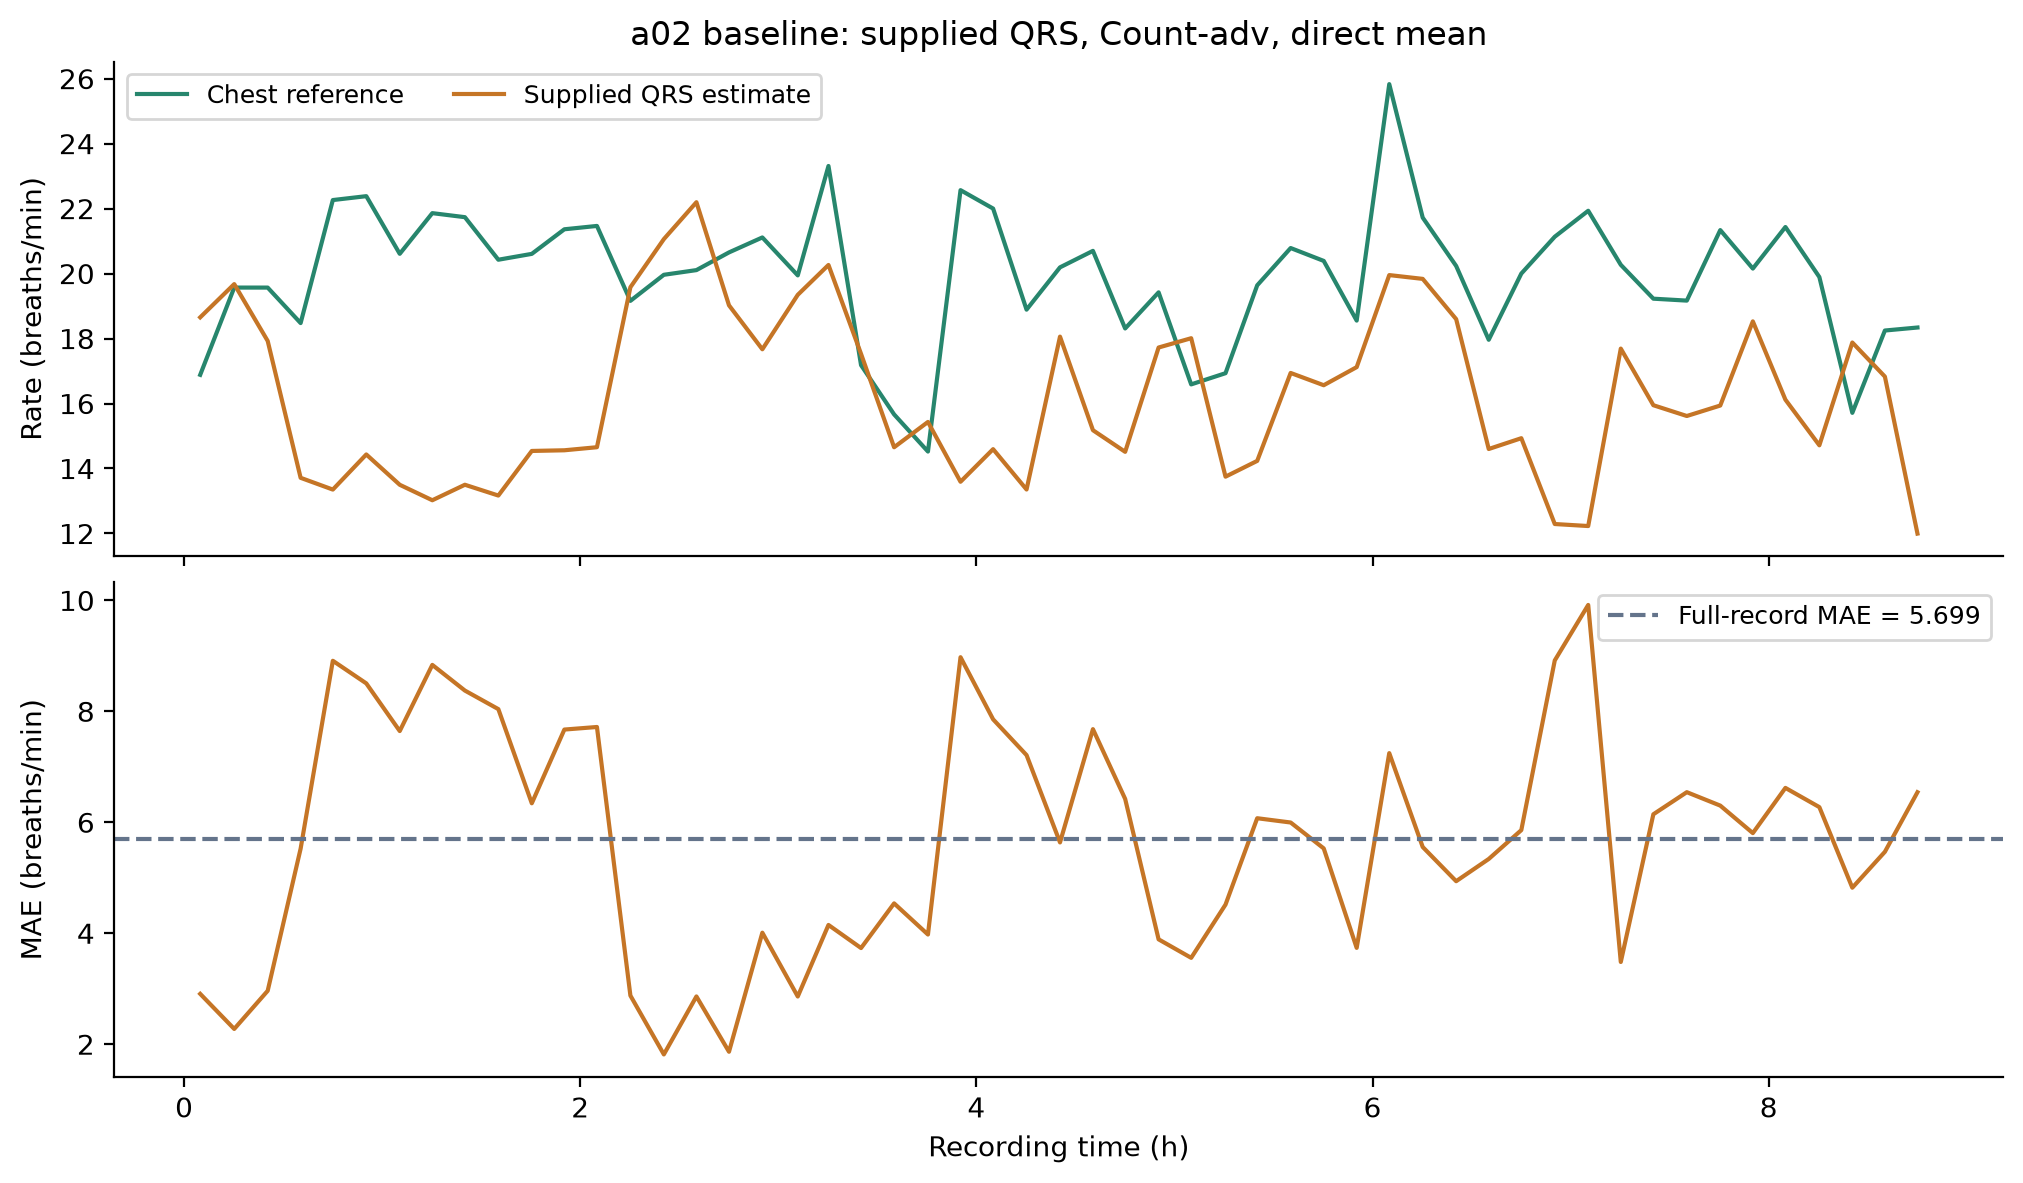
\includegraphics[width=.96\textwidth]{figures/a02_baseline_night.png}\caption{a02 baseline across the night. }\label{fig:baseline_night}\end{figure}

This brings us to the following question regarding the nature of formation of the curves: Is the difference between the two present at the point where chest cycles are detected or is it inherent even in the heartbeat locations?

\subsection{Trace the waveform difference to supplied markers}
Figure~\ref{fig:supplied_gap} displays a02 which is fixed based on time. The visible ECG complexes appear between the supplied markers such that the observed intervals may include more than one visible complex. The baseline mean frequency is 11.95 breaths per minute while the chest-derived reference respiratory rate is 14.29. The longer intervals demonstrate the effect of heartbeats on FM calculation before taking respiratory cycles into account.

\begin{figure}[!htbp]\centering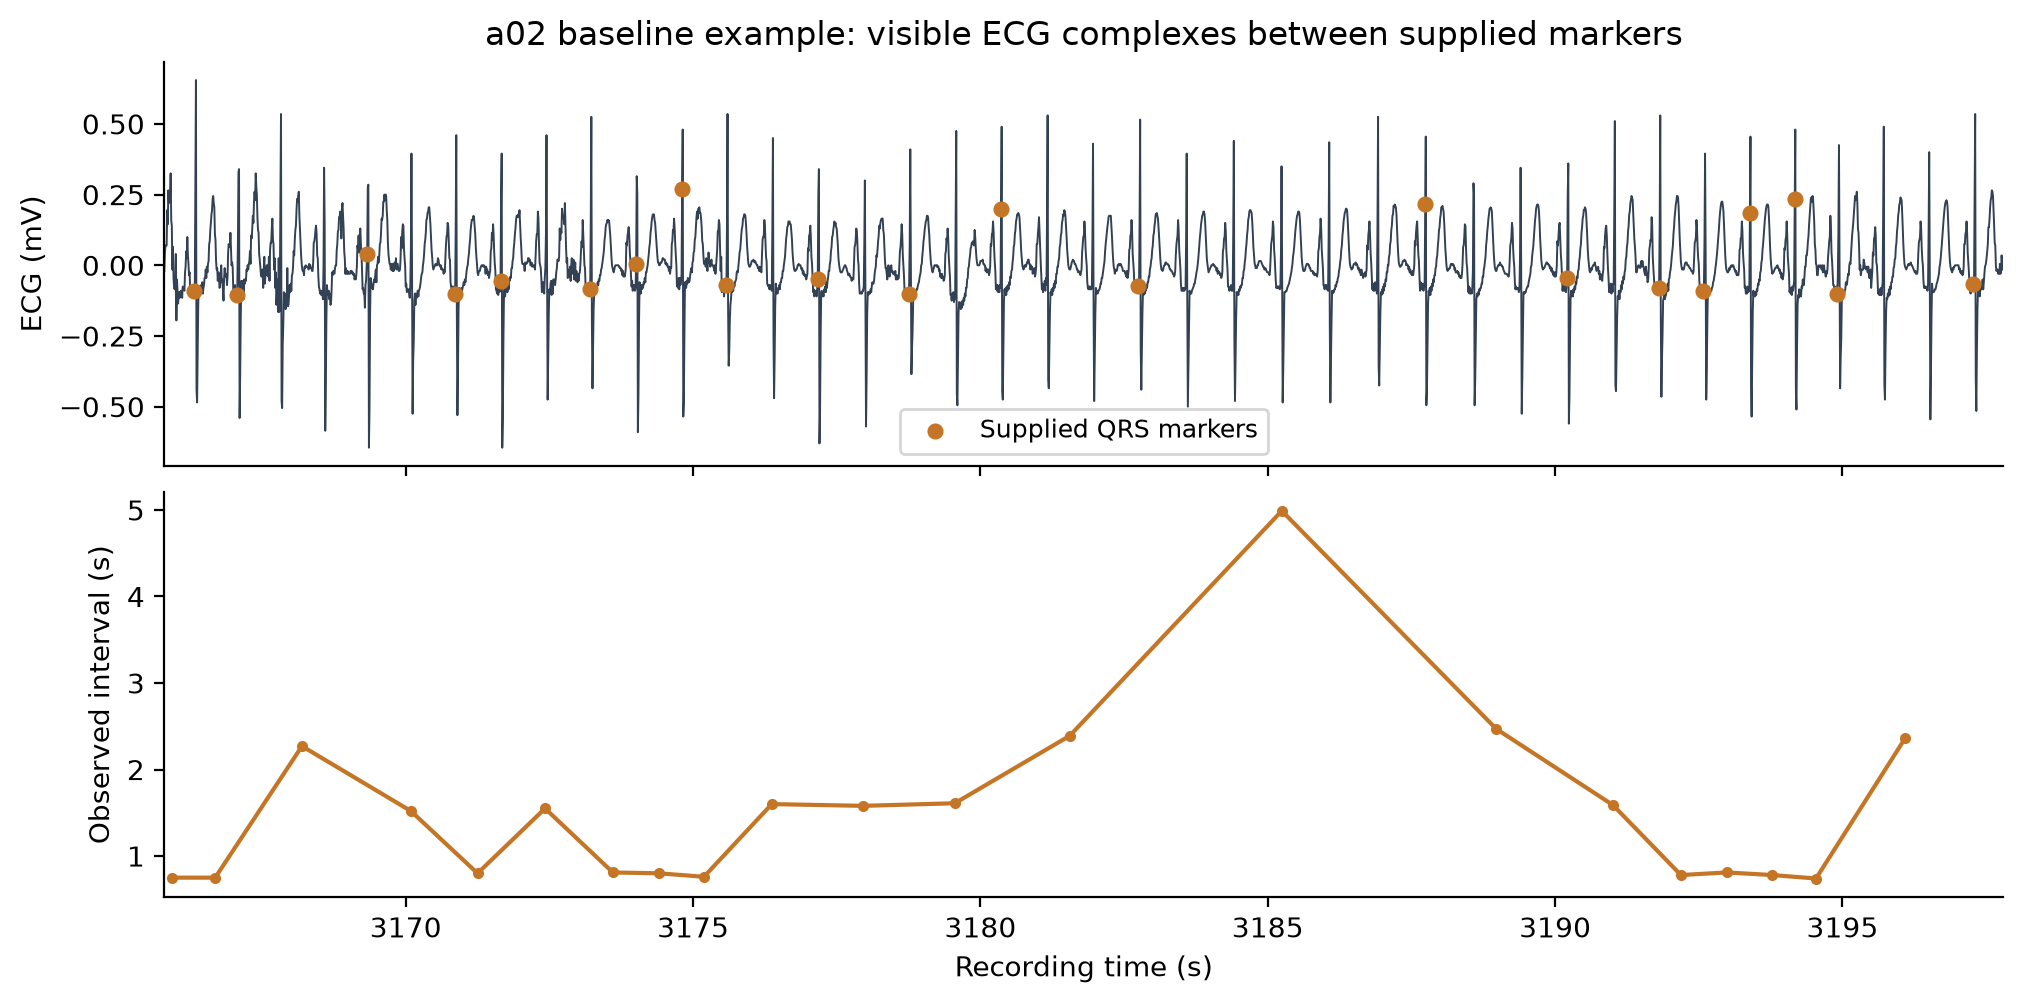
\includegraphics[width=.96\textwidth]{figures/a02_supplied_gap_example.png}\caption{Fixed a02 segment selected by time.}\label{fig:supplied_gap}\end{figure}

The lack of marker means no local amplitude nor baseline calculation. Thus, the problem in the source may appear in all three respiratory clues. In a02, the source includes 35,152 markers and has maximum intervals equal to 13.70 seconds; some longer intervals are explained by local waveforms.

It leads us to the rationale for the following experiment; the detection of heartbeats from the same raw ECG signal and their passing through the respiration processing line. Consequently, in the next chapter, the QRS complex is used to detect the heartbeats in the raw ECG signal again and run the same estimation of respiratory rate.

\FloatBarrier
\newpage

\section{Introduce of GQRS}
\subsection{What GQRS changes?}
To assess the effect of heartbeat markers on the accuracy of respiratory rate estimates, we used the GQRS heartbeat detector algorithm to identify heartbeat positions from the same ECG data set that was used for the experiments in Chapter 2. The GQRS positions were then incorporated into the respiratory rate estimation procedure as described in Chapter 2.

Figure \ref{fig:detector_difference} shows the comparison of both marker types in the same segment as was used in Chapter 3. GQRS uses the position within some longer intervals provided, and therefore modifies the sequence of observed intervals. This new input can therefore be seen directly on the ECG.

\begin{figure}[!htbp]\centering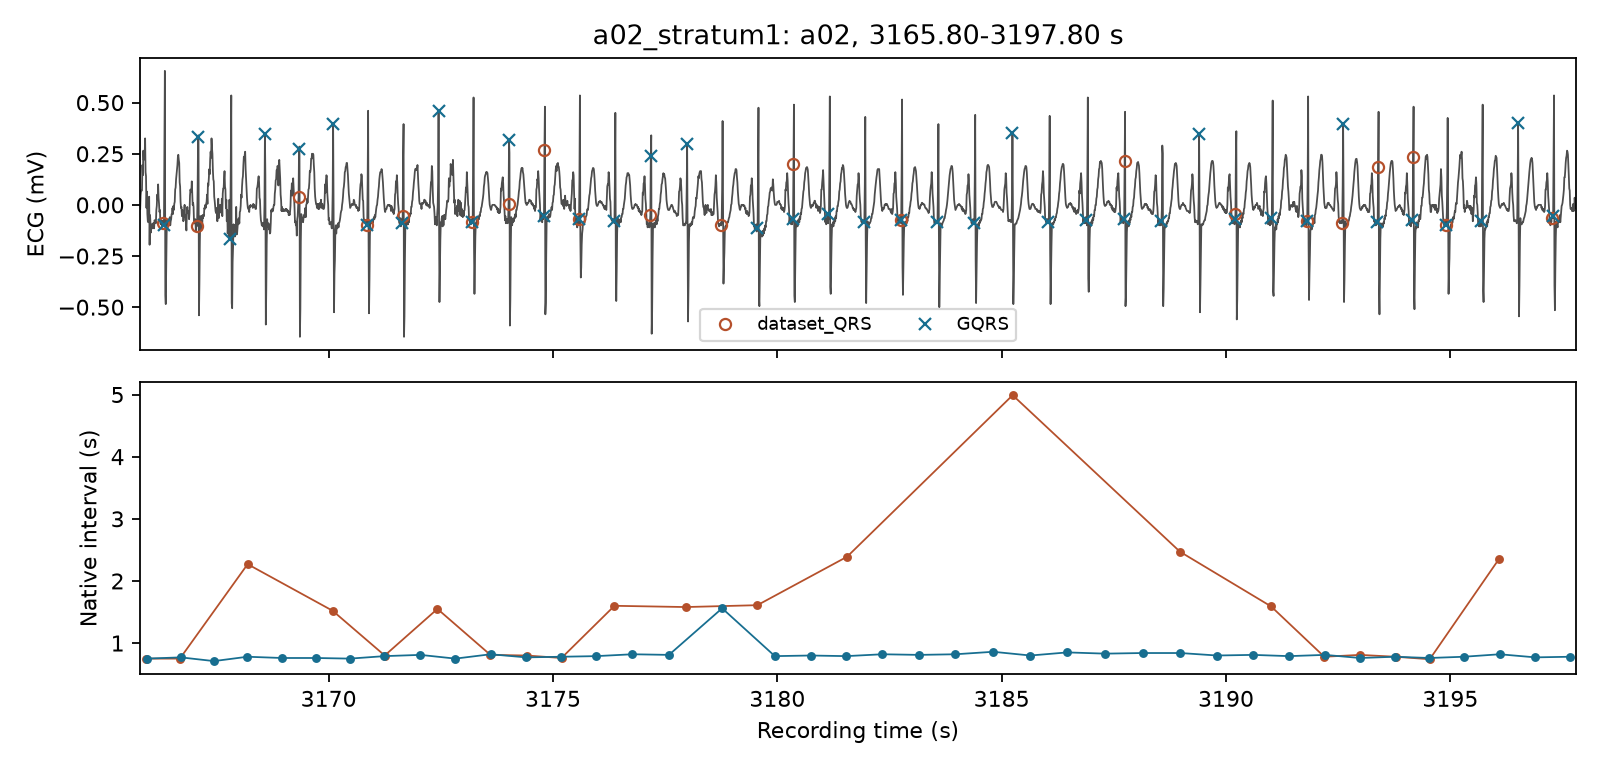
\includegraphics[width=.96\textwidth]{figures/a02_stratum1_beats.png}\caption{The same fixed a02 segment with supplied-QRS and GQRS positions.}\label{fig:detector_difference}\end{figure}

\subsection{Detector settings and the shared processing}
The algorithm GQRS is run once on every complete recording of the ECG data, with the sampling frequency being set at 100 Hz, and the detection threshold set at 1.0, while all other parameters retain their default values. After finding the heartbeat positions, the further processing is done according to the settings defined in Chapter 2, which include a curve at 5 Hz, a 32-second window, two algorithms for cycle counting, and two fusion methods. The reference respiratory rate from the chest does not change.

The original detector times will still be used for FM inputs, but the AM/BW peak-trough times will follow the Chapter 2 conventions. The chest-derived reference respiratory rate times will also stay constant. The orange box in Fig.~\ref{fig:pipeline} will denote the heartbeat input that has been replaced.
\begin{figure}[!htbp]\centering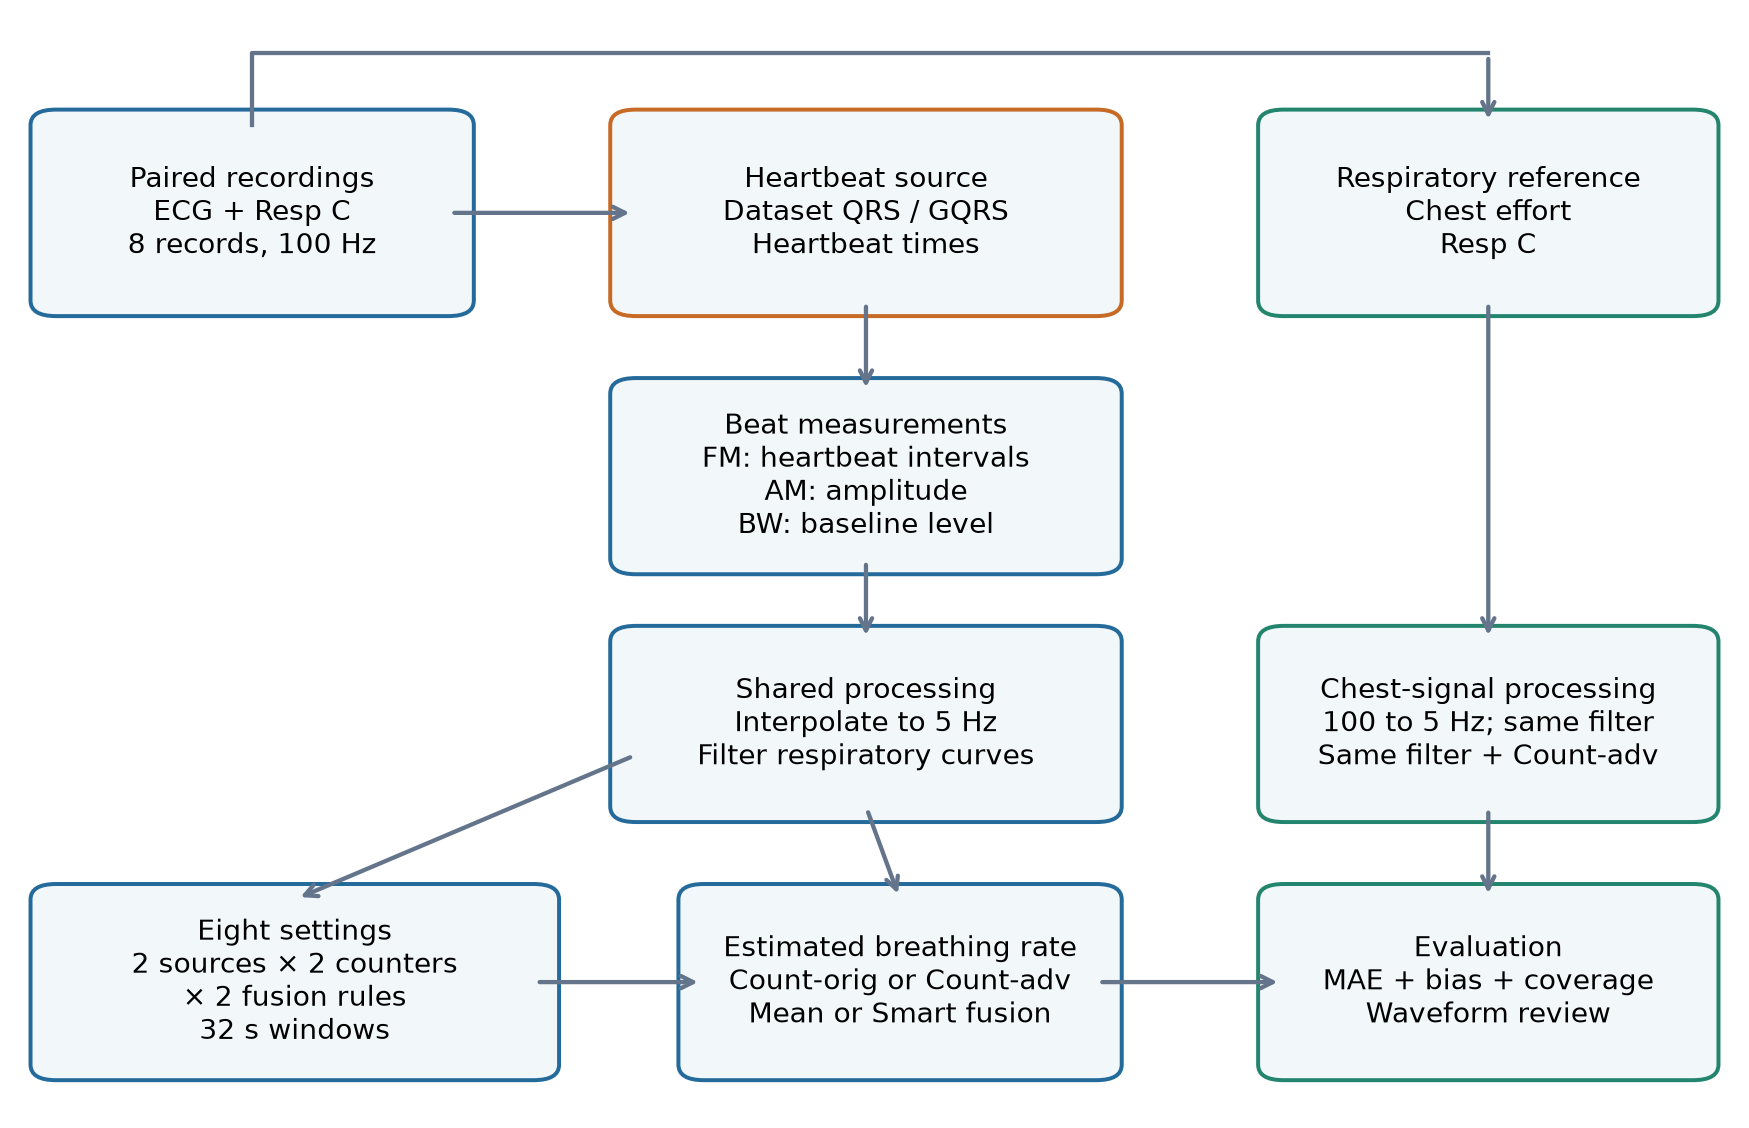
\includegraphics[width=.96\textwidth]{figures/explain_pipeline.png}\caption{Experimental structure and data flow.}\label{fig:pipeline}\end{figure}
\subsection{Results of GQRS experience}
Table~\ref{tab:gqrs} gives the four GQRS outputs. Count-adv with the direct mean gives MAE 3.218 breaths/min on 7,288 paired segments; Smart fusion gives 3.023 on 5,500. Count-orig gives 4.580 and 3.914. The final comparison next uses the same time segments under both sources and examines a02 across its complete recording.

\begin{table}[!htbp]\centering\small\begin{tabular}{llrrr}\toprule Counter & Fusion & Paired windows & Coverage (\%) & MAE\\\midrule
adv & mean & 7,288 & 98.08 & 3.218\\
adv & smart & 5,500 & 74.01 & 3.023\\
orig & mean & 6,891 & 92.73 & 4.580\\
orig & smart & 4,937 & 66.44 & 3.914\\
\bottomrule\end{tabular}\caption{GQRS outputs after rerunning the Chapter 2 pipeline.}\label{tab:gqrs}\end{table}


\FloatBarrier
\newpage

\section{Final comparison: overall change and improvement in a02}
\subsection{Overall results across eight settings}
Table~\ref{tab:overall} places the two runs together. Count-adv direct-mean own-output MAE falls from 3.412 to 3.218 breaths/min at nearly identical coverage. Smart fusion changes from 3.206 to 3.023, with coverage increasing from 71.12\% to 74.01\%. Figure~\ref{fig:overall_comparison} shows both error and available output.

\begin{table}[!htbp]\centering\small\begin{tabular}{lllrrrr}
\toprule
Source & Counter & Fusion & $P$ & $100P/N$ & MAE & Bias \\
\midrule
dataset QRS & adv & mean & 7289 & 98.09 & 3.412 & -0.327 \\
dataset QRS & adv & smart & 5285 & 71.12 & 3.206 & -0.541 \\
dataset QRS & orig & mean & 6820 & 91.78 & 4.422 & 2.877 \\
dataset QRS & orig & smart & 4776 & 64.27 & 3.825 & 2.171 \\
GQRS & adv & mean & 7288 & 98.08 & 3.218 & 0.187 \\
GQRS & adv & smart & 5500 & 74.01 & 3.023 & -0.073 \\
GQRS & orig & mean & 6891 & 92.73 & 4.580 & 3.518 \\
GQRS & orig & smart & 4937 & 66.44 & 3.914 & 2.804 \\
\bottomrule
\end{tabular}
\caption{All eight settings output}\label{tab:overall}\end{table}


\begin{figure}[!htbp]\centering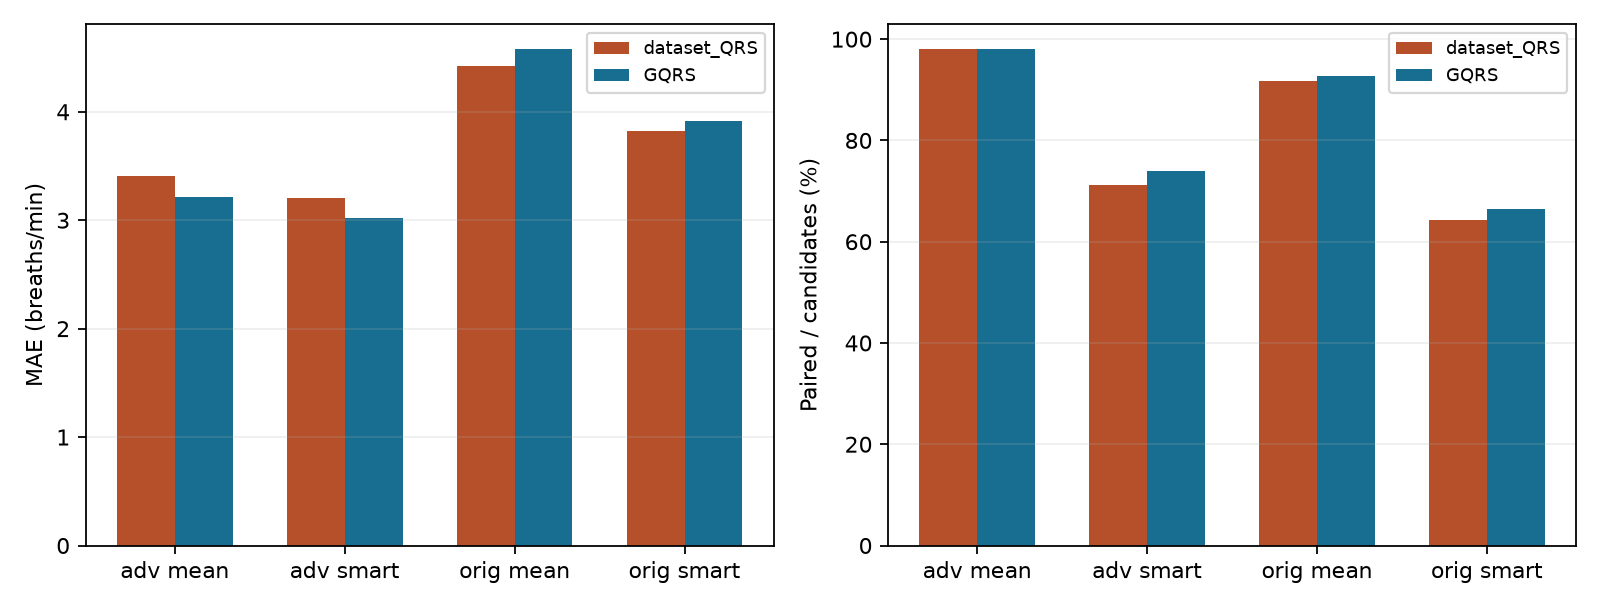
\includegraphics[width=.96\textwidth]{figures/overall.png}\caption{MAE and coverage for the eight source, counter and combination settings.}\label{fig:overall_comparison}\end{figure}

The same-segment source comparisons in Table~\ref{tab:common} retain this direction. Count-adv direct mean changes from 3.412 to 3.218 breaths/min on 7,287 shared segments; Smart fusion changes from 3.084 to 2.909 on 4,793. 

\begin{table}[!htbp]\centering\small\begin{tabular}{lrrrr}
\toprule
Configuration & $P$ & QRS MAE & GQRS MAE & $\Delta$ MAE \\
\midrule
adv mean & 7287 & 3.412 & 3.218 & -0.194 \\
adv smart & 4793 & 3.084 & 2.909 & -0.175 \\
orig mean & 6628 & 4.396 & 4.523 & +0.127 \\
orig smart & 4163 & 3.508 & 3.567 & +0.059 \\
\bottomrule
\end{tabular}
\caption{Same-setting source comparisons on shared windows.}\label{tab:common}\end{table}


\begin{table}[!htbp]\centering\small\begin{tabular}{lrrrr}
\toprule
Record & adv mean & adv smart & orig mean & orig smart \\
\midrule
a01 & 3.69/3.72 & 3.46/3.49 & 2.40/2.39 & 2.09/2.10 \\
a02 & 5.70/4.28 & 6.24/4.49 & 5.58/6.11 & 5.53/5.58 \\
a03 & 4.17/4.00 & 3.76/3.63 & 6.19/6.08 & 4.79/4.64 \\
a04 & 3.88/3.87 & 3.95/3.93 & 4.89/4.92 & 4.59/4.61 \\
b01 & 3.11/3.10 & 2.34/2.37 & 6.11/6.16 & 4.77/4.81 \\
c01 & 1.61/1.78 & 1.44/1.52 & 3.04/3.47 & 2.52/2.83 \\
c02 & 2.67/2.66 & 2.15/2.17 & 5.07/5.19 & 4.19/4.33 \\
c03 & 2.12/2.11 & 2.13/2.11 & 1.61/1.61 & 1.40/1.38 \\
\bottomrule
\end{tabular}
\caption{Per-record shared-window MAE. Each cell is supplied QRS / GQRS, in breaths/min.}\label{tab:records}\end{table}


\begin{figure}[!htbp]\centering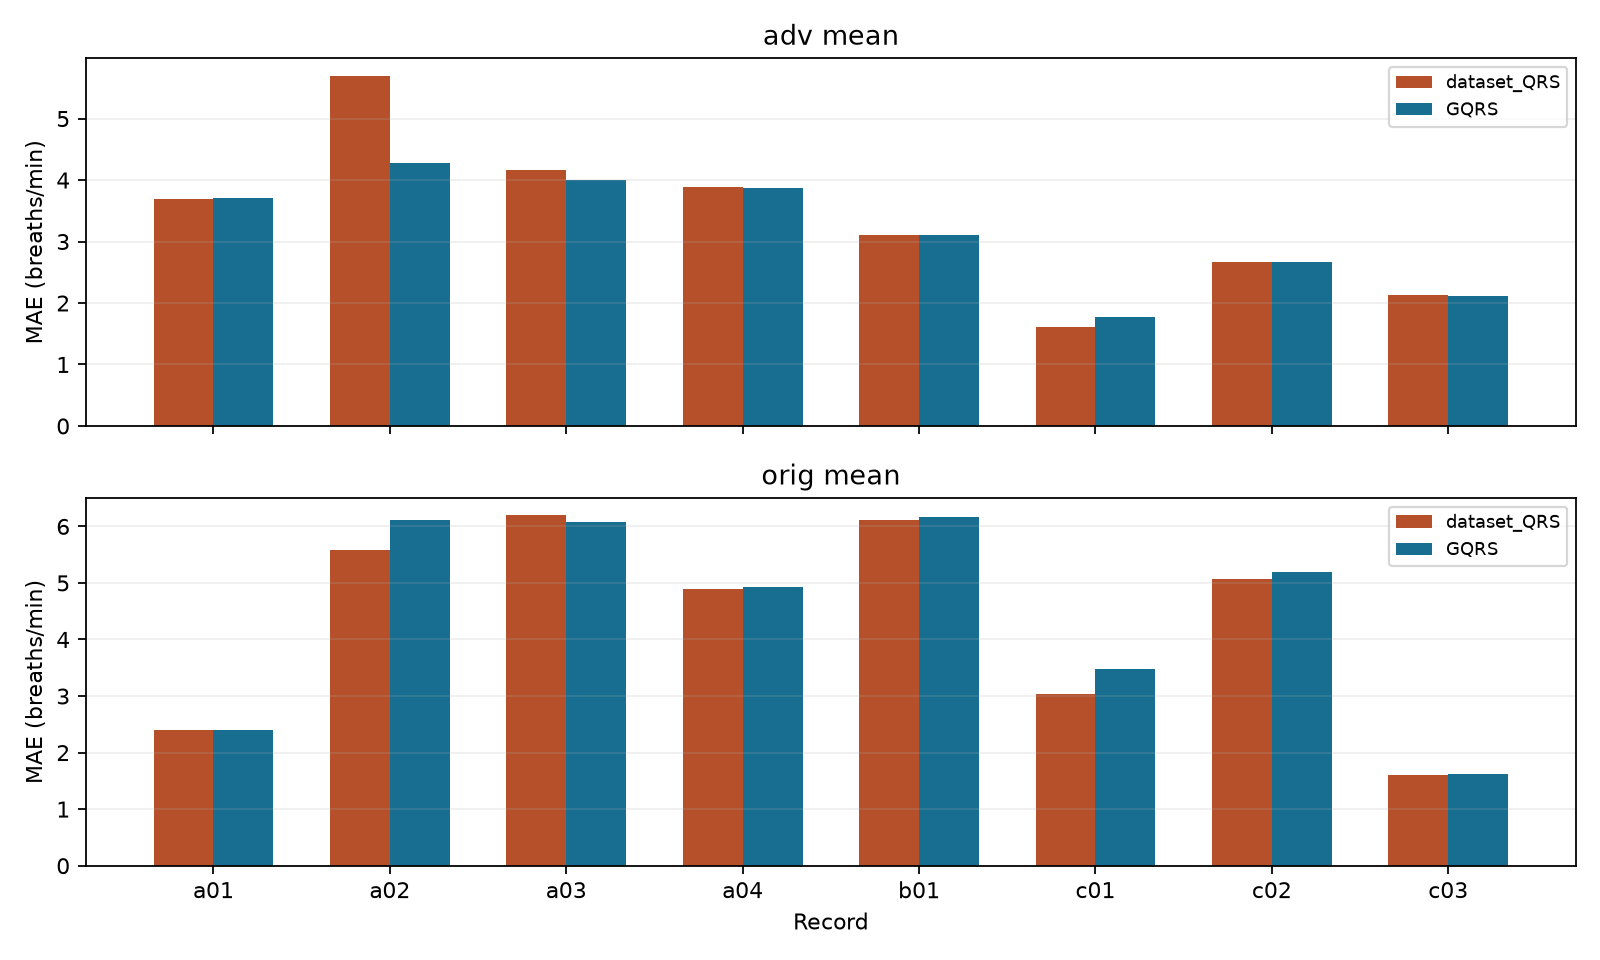
\includegraphics[width=.96\textwidth]{figures/records_common.png}\caption{Per-record shared-window comparison for the direct mean under both cycle-counting methods.}\end{figure}

\FloatBarrier
\subsection{How the complete a02 recording changes}
The most significant record-level enhancement takes place in a02. On the same 982 segments, Count-adv direct-mean MAE goes down from 5.699 to 4.280 breaths/min, which is a reduction by approximately 24.9\%; bias decreases from $-3.747$ to $-0.244$. The error improves in 603 segments, gets worse in 373 and stays the same in six. These numbers characterize the distribution on the recording with its best local instance.

Figure~\ref{fig:night_intervals} comes back to R-R intervals through the night. Position counts go up from 35,152 to 42,382 and the largest interval from 13.70 to 1.69 s. Long jumps in the given sequence are considerably cut down, giving more continuity in R-R intervals to look for the respiratory clues.

\begin{figure}[!htbp]\centering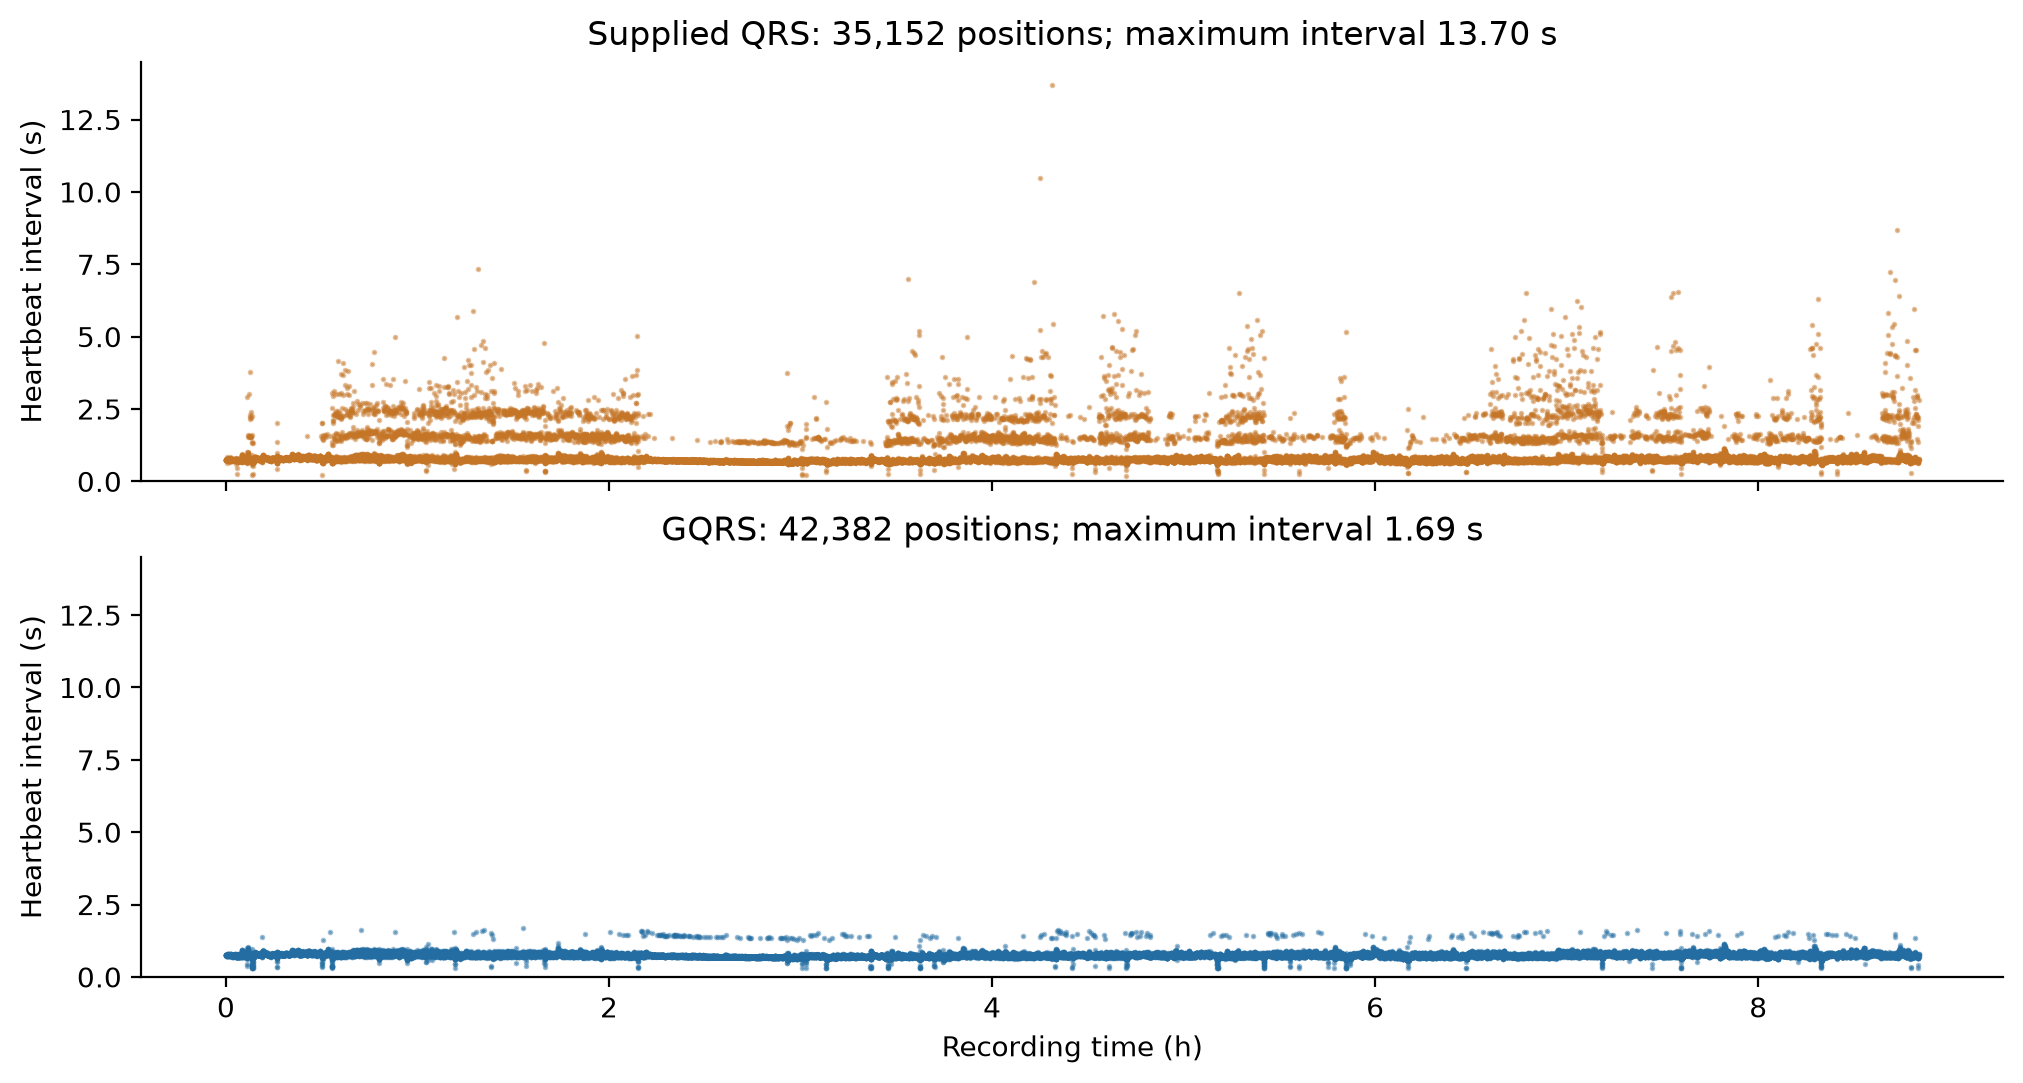
\includegraphics[width=.96\textwidth]{figures/a02_full_record_intervals.png}\caption{All original R-R intervals across a02.}\label{fig:night_intervals}\end{figure}

The figure~\ref{fig:night_comparison} extends the trend into respiratory rates, where the first part is comparing the chest vs ECG-derived respiratory rate, the second part compares the error magnitude over time, and the last one aggregates the segments to compute the resulting MAEs of 5.699 and 4.280. The 10-minute windows used here are for visualization purposes and not for evaluation purposes; the latter uses the 32 seconds intervals as in Chapter 2.

\begin{figure}[!htbp]\centering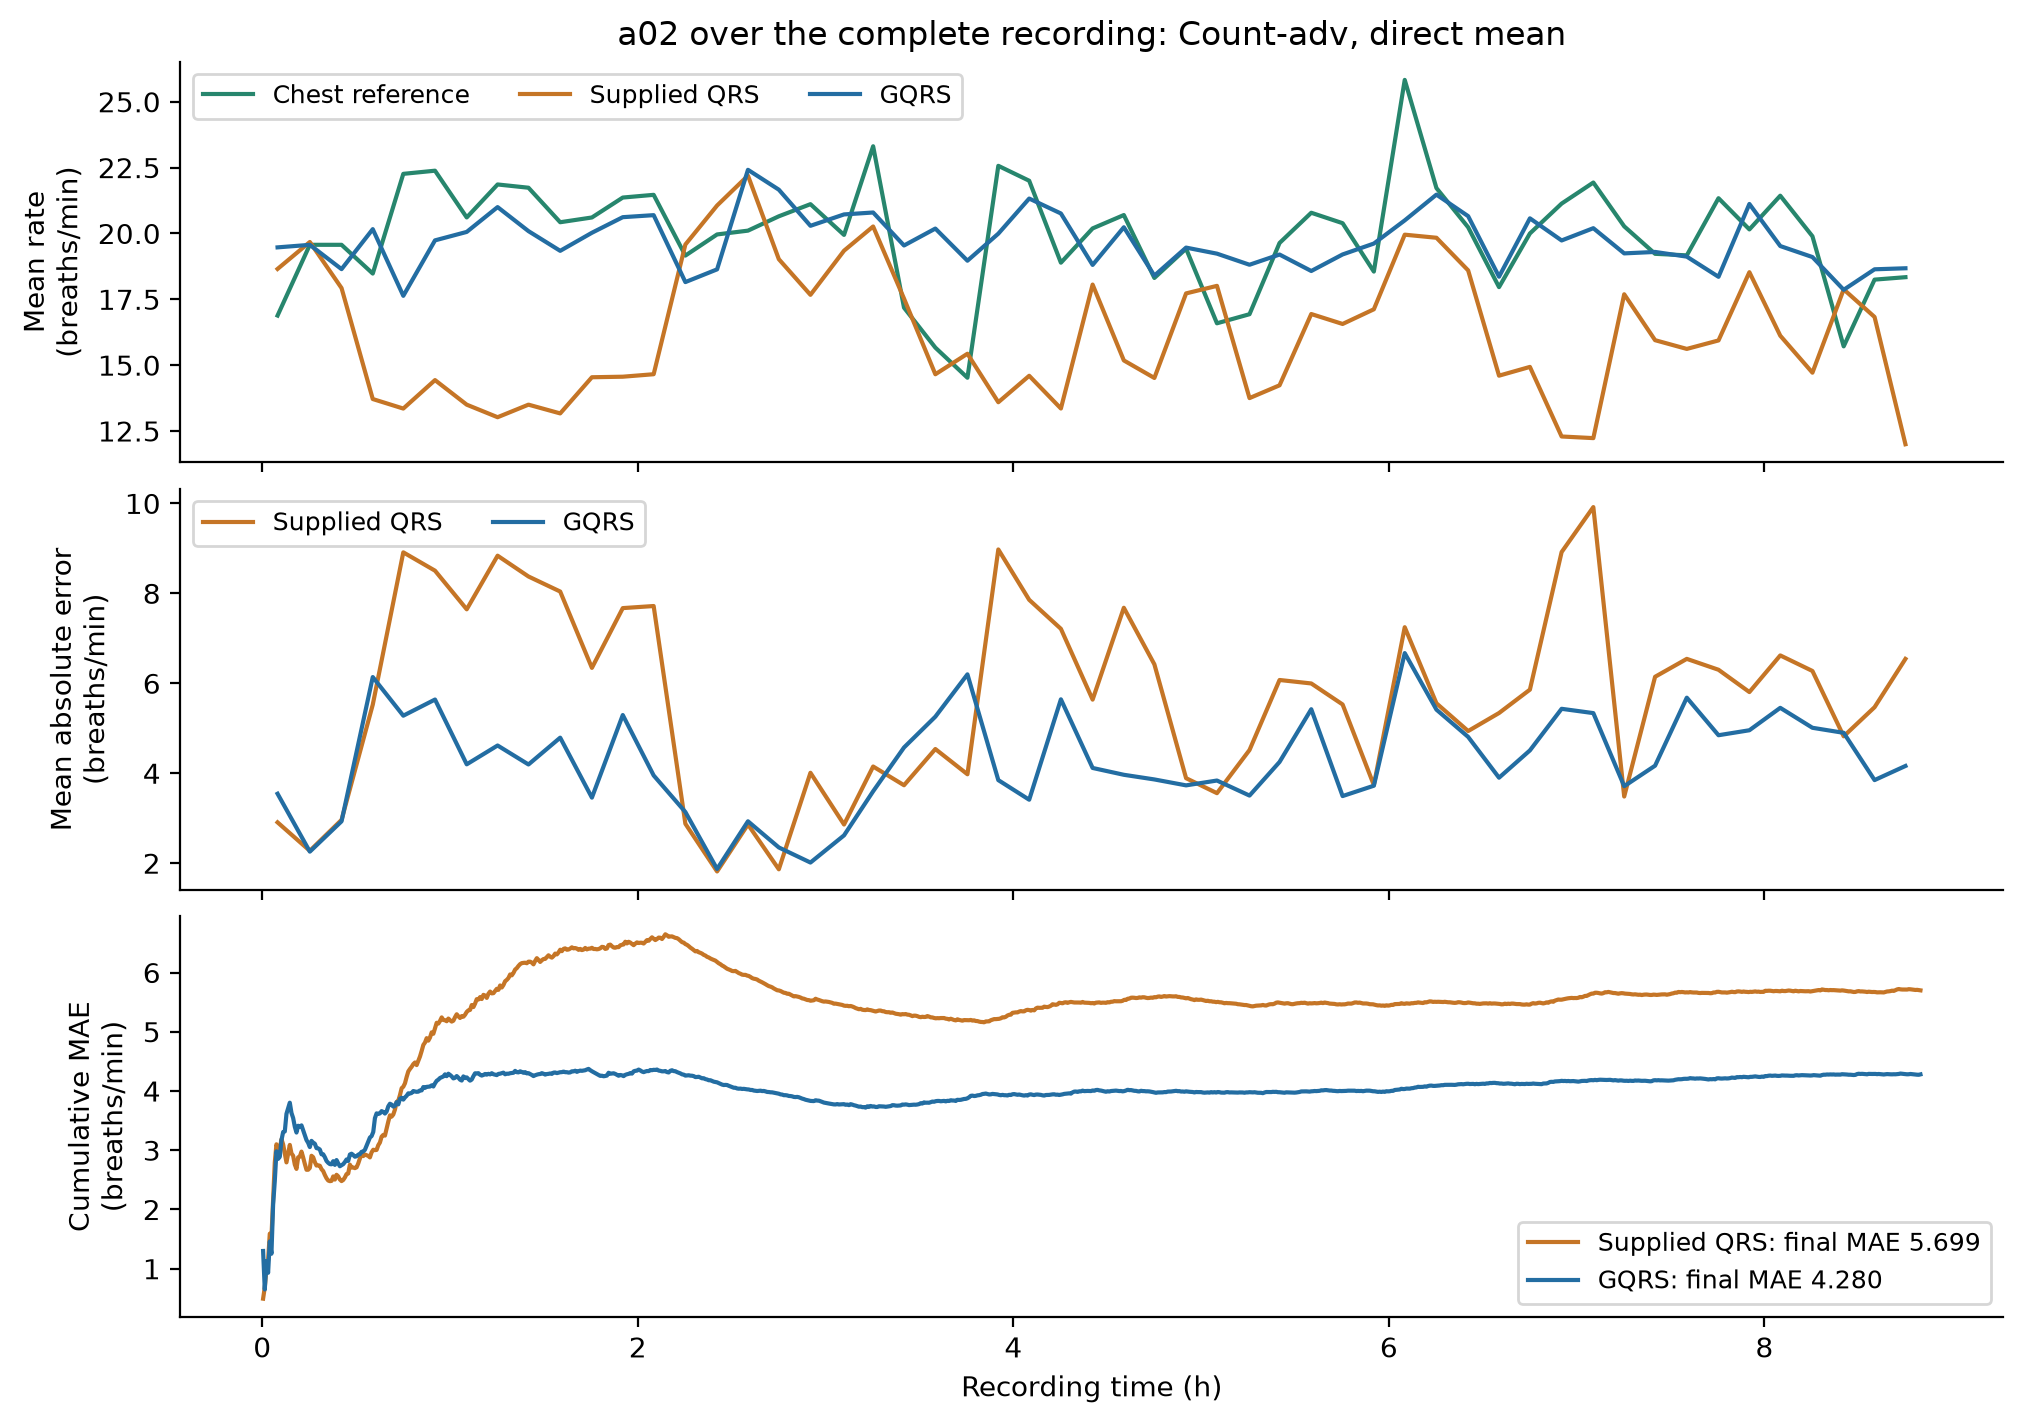
\includegraphics[width=.96\textwidth]{figures/a02_full_record_comparison.png}\caption{a02 on the same 982 paired segments.}\label{fig:night_comparison}\end{figure}

The corresponding numbers for a02 own outputs, using the Smart-fusion paired segments, go from 609 to 718, from 61.27\% to 72.23\%, and from 5.997 to 4.341 breaths/min. The changes at the level of the recordings therefore involve error and bias.

\FloatBarrier
\subsection{How local waveforms explain the recording-level change}
The following additional case exaggerates the effect. It uses the project selection criterion that yields the maximum improvement of Count-adv direct-mean error on common intervals. For 15,264–15,296 s in a02, supplied intervals are about 1.4–2.9 s, whereas GQRS intervals are about 0.7–0.8 s. Complexes are seen in between supplied markers in the original ECG.

\begin{figure}[!htbp]\centering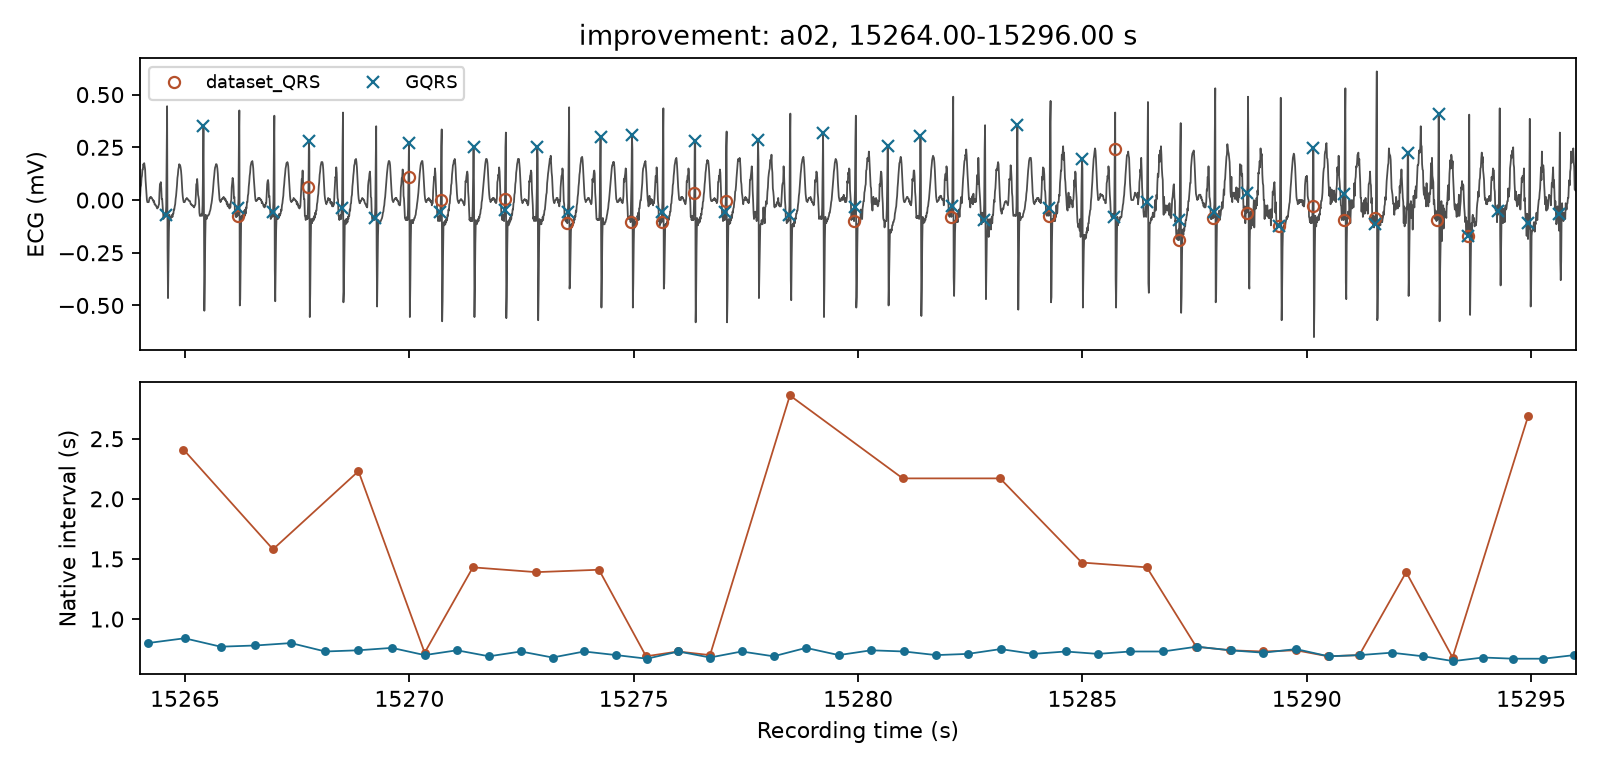
\includegraphics[width=.96\textwidth]{figures/improvement_beats.png}\caption{Maximum adv/mean improvement: detected positions and intervals.}\end{figure}

FM/AM/BW respiratory rate shift from 8.89/14.85/11.72 to 31.11/25.49/28.38 breaths/min. Their mean value shifts from 11.82 to 28.33 compared to 29.51 as chest-derived reference respiratory rate, reducing absolute error by 16.51. The curves demonstrate how replacement of sources modifies intervals and amplitude and baseline cycles around beats.

\begin{figure}[!htbp]\centering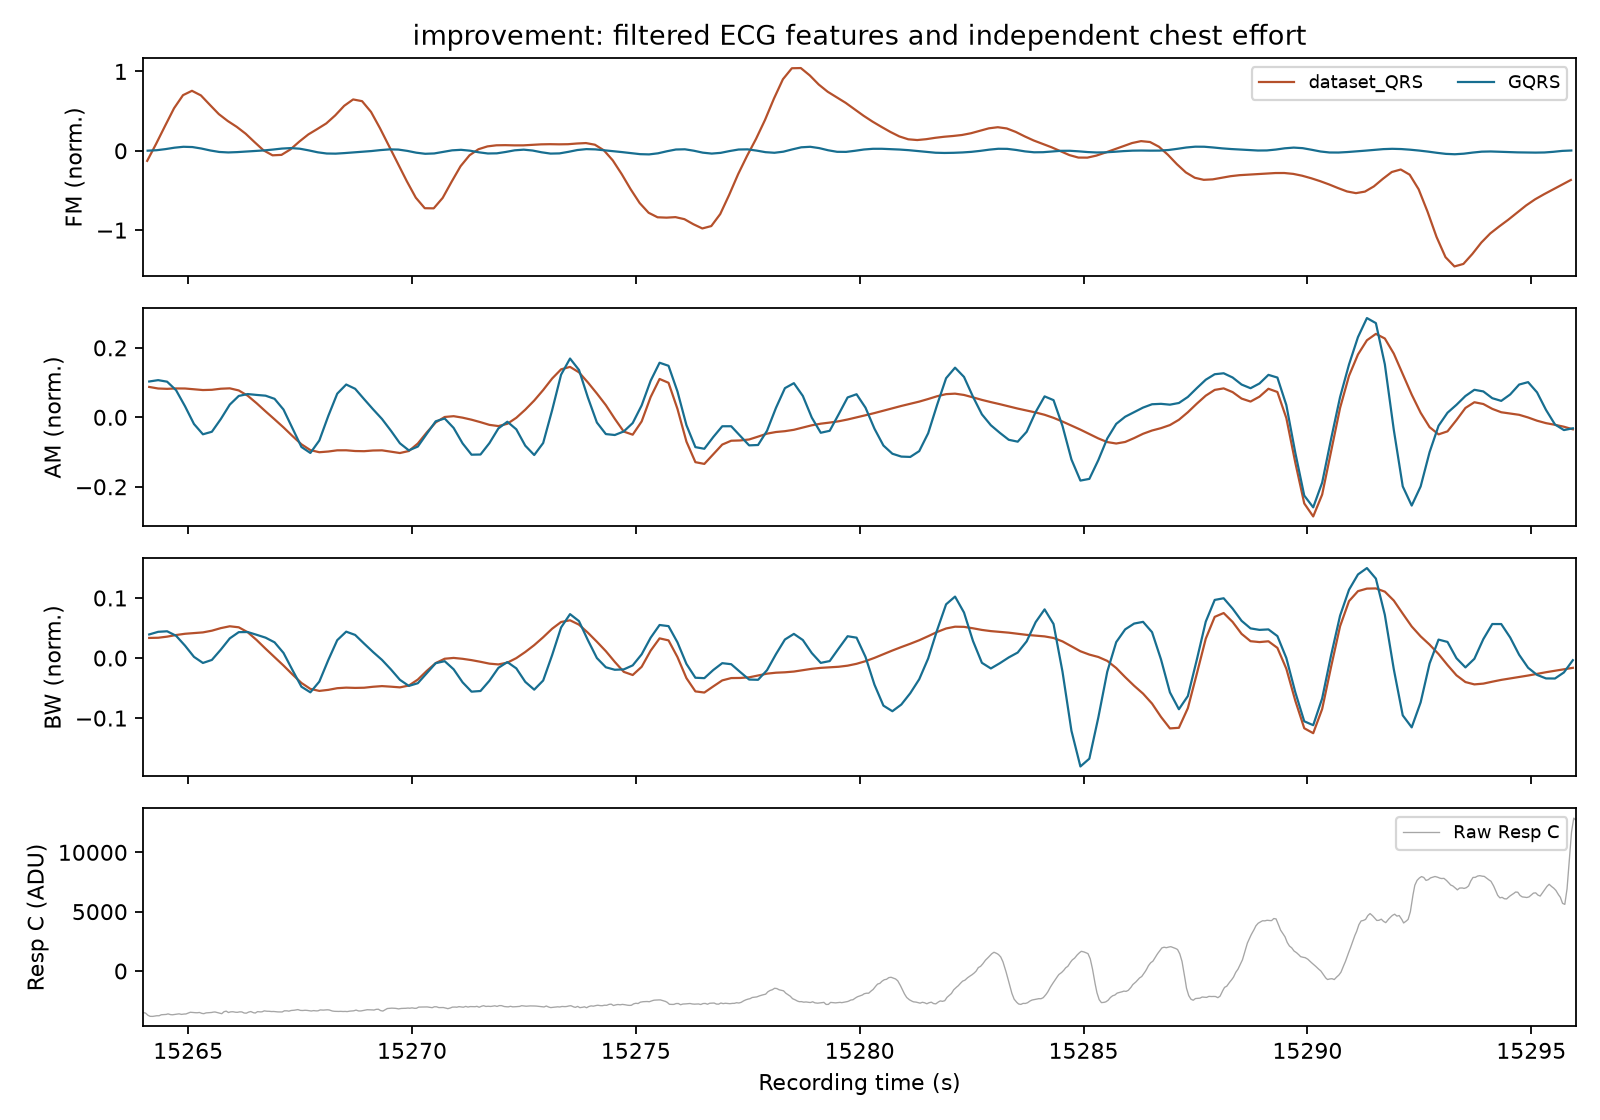
\includegraphics[width=.96\textwidth]{figures/improvement_features.png}\caption{The same improvement segment: separate FM, AM and BW features with raw chest effort.}\end{figure}
Resp C is weaker initially and stronger eventually, with reference cycles provided primarily by the oscillations which are retained eventually. The reading of the reference against the ECG characteristics makes the connection in this regard because of altered positions, altered curves, altered number of cycles.
\begin{figure}[!htbp]\centering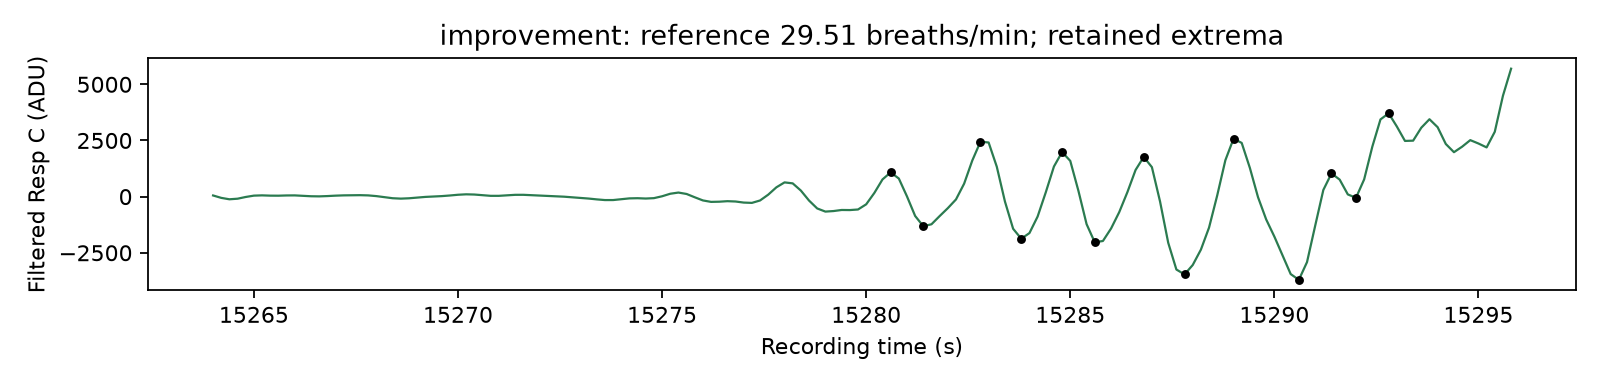
\includegraphics[width=.96\textwidth]{figures/improvement_reference.png}\caption{Retained chest extrema in the improvement segment.}\end{figure}

\FloatBarrier
\subsection{Complete interpretation and conclusion}
The improvements to a02 are evident in both recordings and local waveform analysis. Other recordings show smaller changes in opposite directions: the a03 common window Count-adv direct-mean MAE varies from 4.170 to 4.002 breaths/min, whereas c01 moves from 1.612 to 1.777. The two Count-orig common window MAEs vary from 4.396/3.508 to 4.523/3.567 (Table~\ref{tab:common}). Thus the choice of cycles influences the source comparison as well.

The novel contribution in this work is in the connected approach: starting with QRS discrepancies for provided data, detecting marker problems in raw waveforms, and repeating the whole respiratory analysis based on independent cycle detections. Based on the Count-adv method, the most important part of pooled improvement comes from a02.



% End body
\FloatBarrier\clearpage\phantomsection\addcontentsline{toc}{section}{References}\bibliographystyle{unsrtnat}\bibliography{references}
\bigskip
\section*{AI Use Declaration}\addcontentsline{toc}{section}{AI Tool Use Declaration}
OpenAI Codex assisted with Python code implementation,  report outline , translation and document layout. 
\end{document}
